\documentclass[9pt, a4paper]{article}

\usepackage{graphicx}
\usepackage{listings}
\usepackage{color}
\usepackage{amsmath}
\usepackage{geometry}
\usepackage{setspace}
\usepackage{biblatex}
\usepackage{float}
\usepackage[hidelinks]{hyperref}
\usepackage{subcaption}
\usepackage[export]{adjustbox}
\usepackage[normalem]{ulem}
\usepackage{wrapfig}
\usepackage{gensymb}
\usepackage{caption}

\addbibresource{citations.bib}
 
% Page master configuration
\lstset { basicstyle=\ttfamily, breaklines = true, tabsize=2 }
\geometry { a4paper, total={170mm,257mm}, left=20mm, top=20mm, right=20mm, bottom=20mm }
\graphicspath{{Images/}}
\addbibresource{biblography.bib}
\setlength{\parskip}{0.5em}
\setlength{\parindent}{0cm}
\setlength{\belowcaptionskip}{-10pt}

\definecolor{dkgreen}{rgb}{0,0.6,0}
\definecolor{gray}{rgb}{0.5,0.5,0.5}
\definecolor{mauve}{rgb}{0.58,0,0.82}

\lstset{frame=tb,
  language=Java,
  aboveskip=3mm,
  belowskip=3mm,
  showstringspaces=false,
  columns=flexible,
  basicstyle={\footnotesize\ttfamily},
  numbers=none,
  numberstyle=\tiny\color{gray},
  keywordstyle=\color{blue},
  commentstyle=\color{dkgreen},
  stringstyle=\color{mauve},
  breaklines=true,
  breakatwhitespace=true,
  tabsize=3
}

%%%%%%%%%%%%%%%%%%%%%%%%%%%%%%%%%%%%%%%%%%%%%%%%%%%%%%%%%%%%%%%%%%%%%%%%%%%%%%%%%%%%%%%%%%%%%%%%%%%%%%%%%%
\begin{document}

\begin{titlepage}
	\newcommand{\HRule}{\rule{\linewidth}{0.5mm}}
    
\includegraphics[scale=0.1]{./Images/Imperial_Logo.jpg} 
    \\
    \center 
	\textsc{\large Department of Electrical and Electronic Engineering }\\[0.5cm] 
	\textsc{\normalsize ELEC60030: Robotic Manipulation}\\[0.5cm] 
    
	\HRule \\[0.4cm]
	Team Machina: OpenMANIPULATOR-X Coursework Report
    \HRule \\[1.5cm]
     
    \begin{center}
		\underline{Authors}\\[0.5cm] 
        Khayle Torres \\ CID: 01753211 \\ kt1719@ic.ac.uk \\ [0.5cm]

        Xin Wang \\ CID: 01735253 \\ xw2519@ic.ac.uk \\ [0.5cm]
        
        Yuna Valade \\ CID: 01765409 \\ yv19@ic.ac.uk \\ [0.5cm]

	\end{center} \large

    \vfill 
    \makeatletter
    \@date 
    \makeatother
\end{titlepage}

%%%%%%%%%%%%%%%%%%%%%%%%%%%%%%%%%%%%%%%%%%%%%%%%%%%%%%%%%%%%%%%%%%%%%%%%%%%%%%%%%%%%%%%%%%%%%%%%%%%%%%%%%%
\renewcommand{\baselinestretch}{0.75}\normalsize
\tableofcontents
\renewcommand{\baselinestretch}{1.0}\normalsize

\pagebreak
%%%%%%%%%%%%%%%%%%%%%%%%%%%%%%%%%%%%%%%%%%%%%%%%%%%%%%%%%%%%%%%%%%%%%%%%%%%%%%%%%%%%%%%%%%%%%%%%%%%%%%%%%%

%%%%%%%%%%%%%%%%%%%%%%%%%%%%%%%%%%%%%%%%%%%%%%%%%%%%%%%%%%%%%%%%%%%%%%%%%%%%%%%%%%%%%%%%%%%%%%%%%%%%%%%%%%
\section{Task 1 - Modelling}

\subsection{Assigning Co-ordinate Frames}

The process of assigning the co-ordinate frames and the design decisions taken
are summarised into the following points:
\begin{itemize}
    \item Based on the CAD models \cite{CAD_model} of the robotic arm, the team assigned labels
    to each of the joints as shown in Figure 1(a).  

    \item Where the arm has a joint, the team assigned an inital co-ordinate
    frame to it as shown in Figure 1(b). 
    \begin{figure}[h!]
      \centering
      \begin{subfigure}{.5\textwidth}
        \centering
        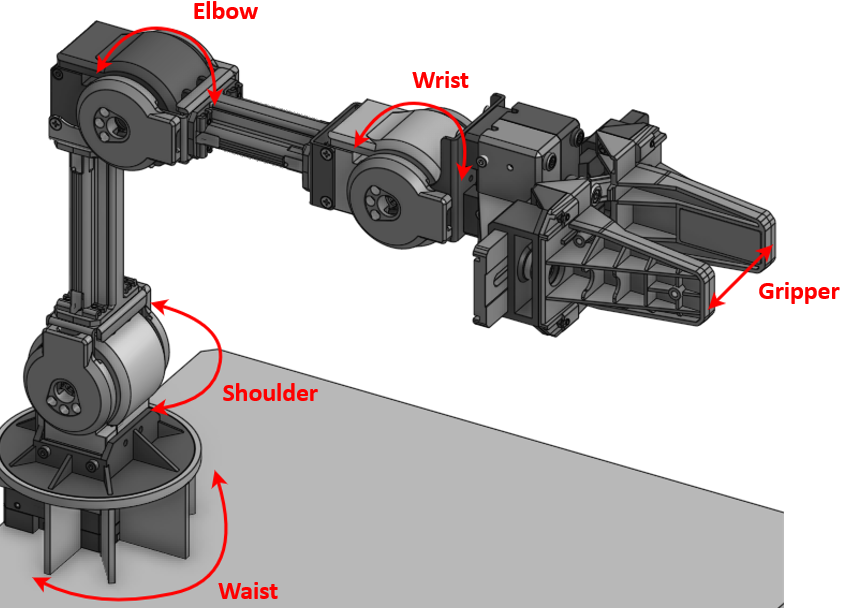
\includegraphics[width=7cm]{Arm diagram.PNG}
        \caption{Location of robotic arm joints and labels}
      \end{subfigure}%
      \begin{subfigure}{.5\textwidth}
        \centering
        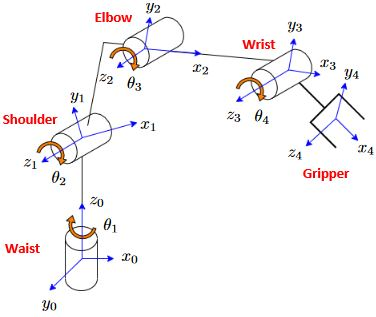
\includegraphics[width=5.9cm]{Coodinate frame.JPG}
        \caption{Initial assigment of co-ordinate frames \cite{Coordinate_frame}}
      \end{subfigure}
      \caption{}
    \end{figure}

    The actual model from which the DH table is generated is modified with the following
    design decisions:

    \begin{minipage}{.45\textwidth}
      \begin{itemize}
        \item The co-ordinate frame for the \textit{Waist} and \textit{Shoulder}
        both have the same height $z$. By setting it to the same height, it
        simplifies the final DH table since we do not have to account for the
        different heights. 
  
        \item There is an offset in the horizontal $x$ axis between the \textit{Shoulder}
        and \textit{Waist} co-ordinate frames as shown on the right. Instead of
        accounting for the $z$-axis offset and $x$-axis offset, the length of
        the hypotenus ($0.130 m$) and the angle subtended ($10.6 \deg$) is used.
        This further simplifies the resulting DH table shown in the next section.
      \end{itemize}
    \end{minipage}
    \begin{minipage}{.45\textwidth}
      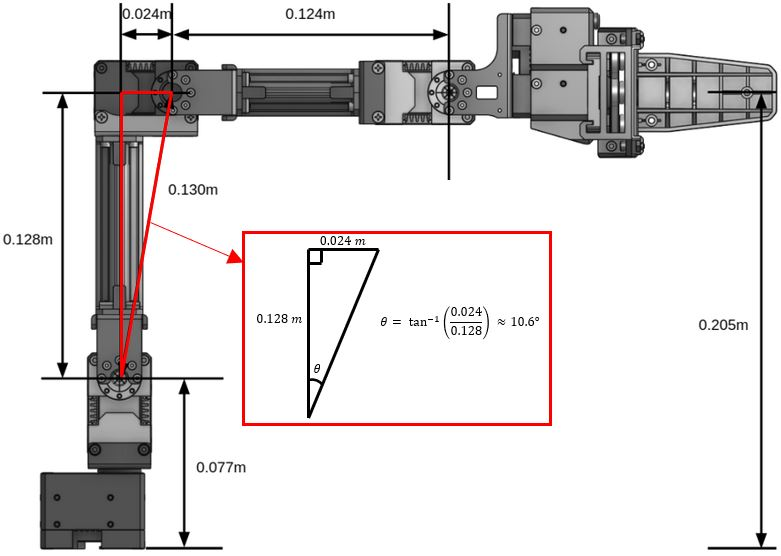
\includegraphics[width=7.5cm]{Offset angle.JPG}
      \captionof{figure}{}

    \end{minipage}
    
    \item The robotic arm's end effector location is designed to be in the center by default but its final position can be changed depending on the task e.g. the end effector location for drawing will be different to the end effector location for interacting with cubes.
    
\end{itemize} 

\subsection{DH Table}
The DH table is created based on the standard robotic arm position as show in Figure 1(a), and the co-ordinate frames for \textit{Waist} and \textit{Shoulder} are in the same location with different orientations.

\begin{table}[h]
    \centering
    \begin{tabular}{|c|c|c|c|c|}
    \hline
    {\textbf{}} & {\textbf{$\alpha_{i-1}$}} & { \textbf{$a_{i-1}$}} & { \textbf{$d_i$}} & { \textbf{$\theta_i$}} \\ \hline
    \textbf{Waist}           & $0 \degree$                          & 0                        & 0.077                & $\theta_1$                \\ \hline
    \textbf{Shoulder}           & $90 \degree$                              & 0                        & 0                    & $\theta_2 + 90\degree - 10.6\degree$    \\ \hline
    \textbf{Elbow}           & $0 \degree$                               & 0.130                    & 0                    & $\theta_3 - 90\degree + 10.6\degree$    \\ \hline
    \textbf{Wrist}           & $0 \degree$                               & 0.124                    & 0                    & $\theta_4$                \\ \hline
    \textbf{Gripper}           & $0 \degree$                               & 0.126                    & 0                    & 0                         \\ \hline
    \end{tabular}
\end{table}

Referring to the \textit{Shoulder} and \textit{Elbow} in the DH table, there are
additions of $+90 \degree - 10.6\degree$ and $-90 \degree + 10.6\degree$ respectively in order to ensure the
standard pose in Figure 2 \cite{CAD_model} is achieved with all joint angles set to $0
\degree$.  $10.6$

\subsection{Forward Kinematics}

With the DH table completed, the Forward Kinematics is implemented by
calculating the transformation matrix for each joint and multiplying them
together. This functionality is implemented as a \verb+trajectoryLib+ class
function that returns $x,y,z$ co-ordinate of the end-effector (\textit{Gripper})
when the angles for each joint is specfied. 

Each frame has it's own transformation matrix that is derived from each row on
the specified DH table above.  Each transformation matrix is relative to
previous frames hence why all transformation matrices are multiplied together.
Each consecutive frame is built on the cumulative rotations and transformations
of all the frames that came before it. The forward kinematic matrices is
shown under \verb+Appendix: Forward Kinematics+

As mentioned previously, this is seen in the following diagrams showing the range of rotations
for each joint with all other joints set to 0.
\begin{figure}[h]
  \centering
  \begin{subfigure}{.5\textwidth}
    \centering
    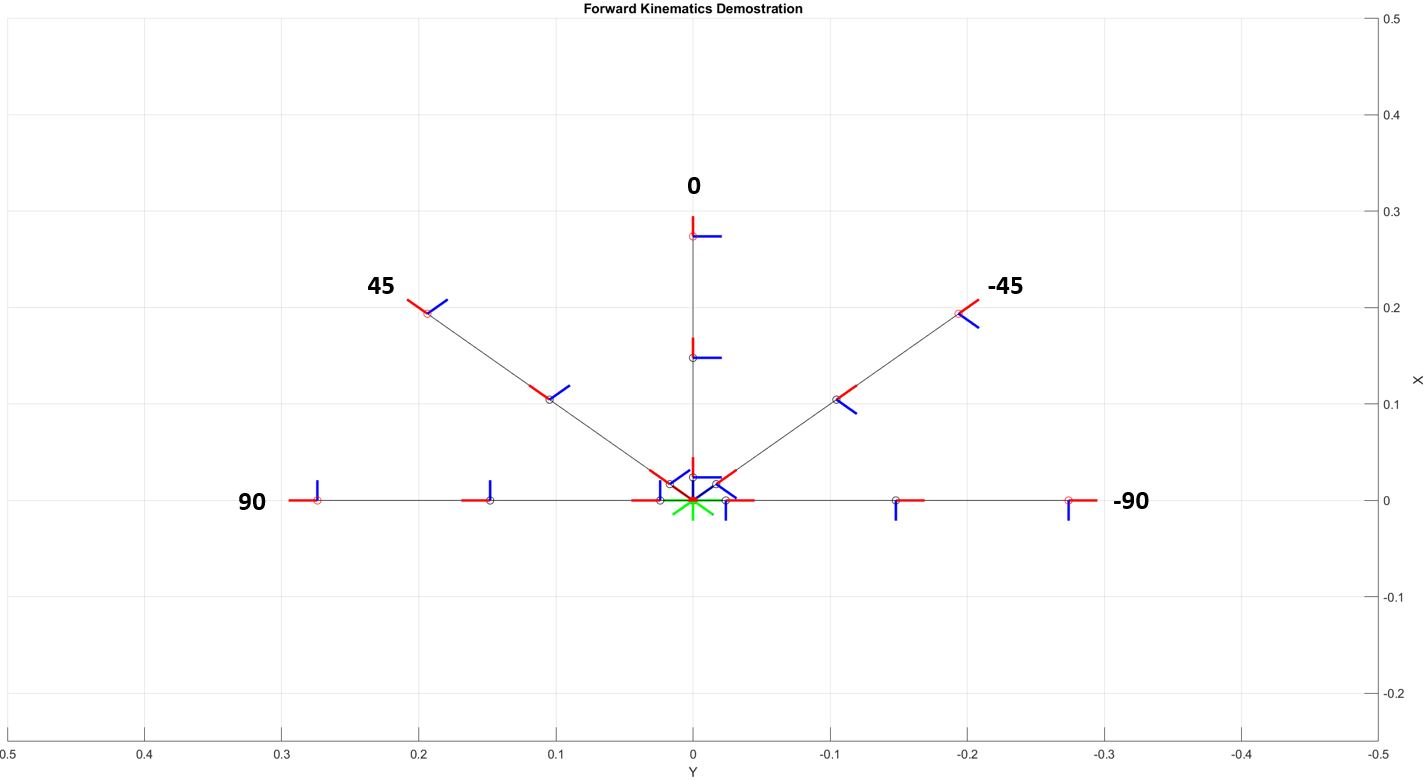
\includegraphics[width=7cm]{theta1.JPG}
    \caption{$\theta_1$ rotation: [$90\degree, 45\degree, 0\degree, -45\degree, -90\degree$]}
  \end{subfigure}%
  \begin{subfigure}{.5\textwidth}
    \centering
    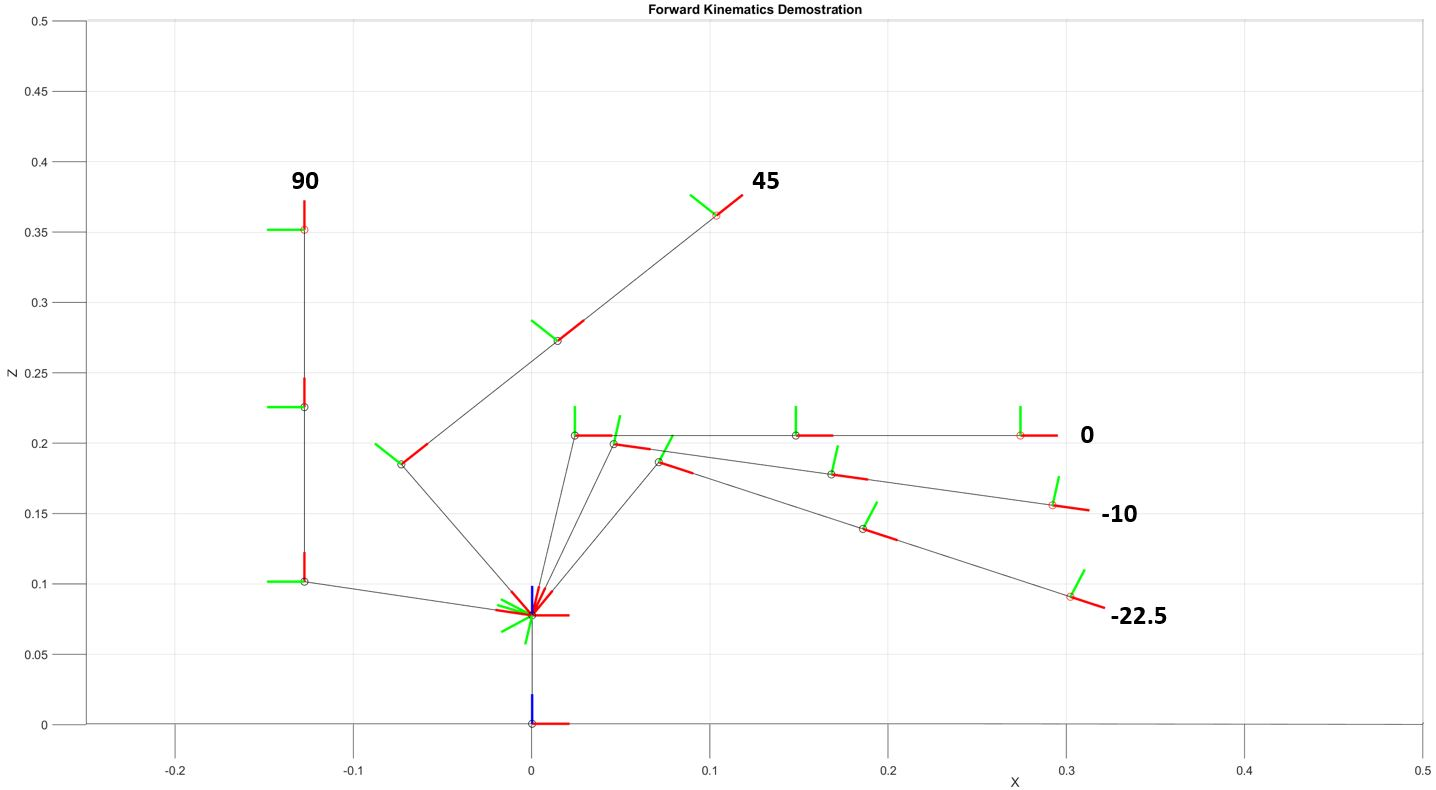
\includegraphics[width=7cm]{theta2.JPG}
    \caption{$\theta_2$ rotation: [$90\degree, 45\degree, 0\degree, -10\degree, -22.5\degree$]}
  \end{subfigure}
\end{figure}
\begin{figure}[h]
  \centering
  \begin{subfigure}{.5\textwidth}
    \centering
    \addtocounter{subfigure}{2}
    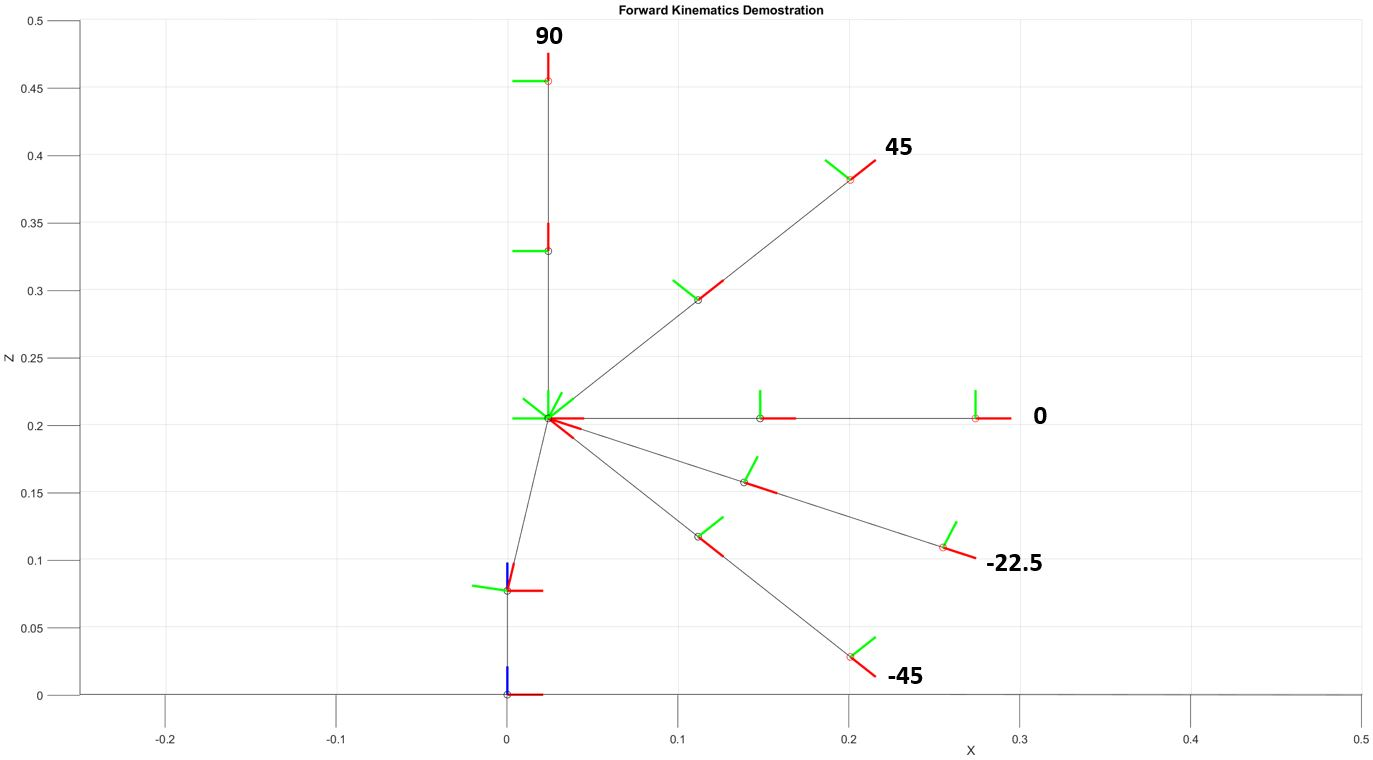
\includegraphics[width=7cm]{theta3.JPG}
    \caption{$\theta_3$ rotation: [$90\degree, 45\degree, 0\degree, -22.5\degree, -45\degree$]}
  \end{subfigure}%
  \begin{subfigure}{.5\textwidth}
    \centering
    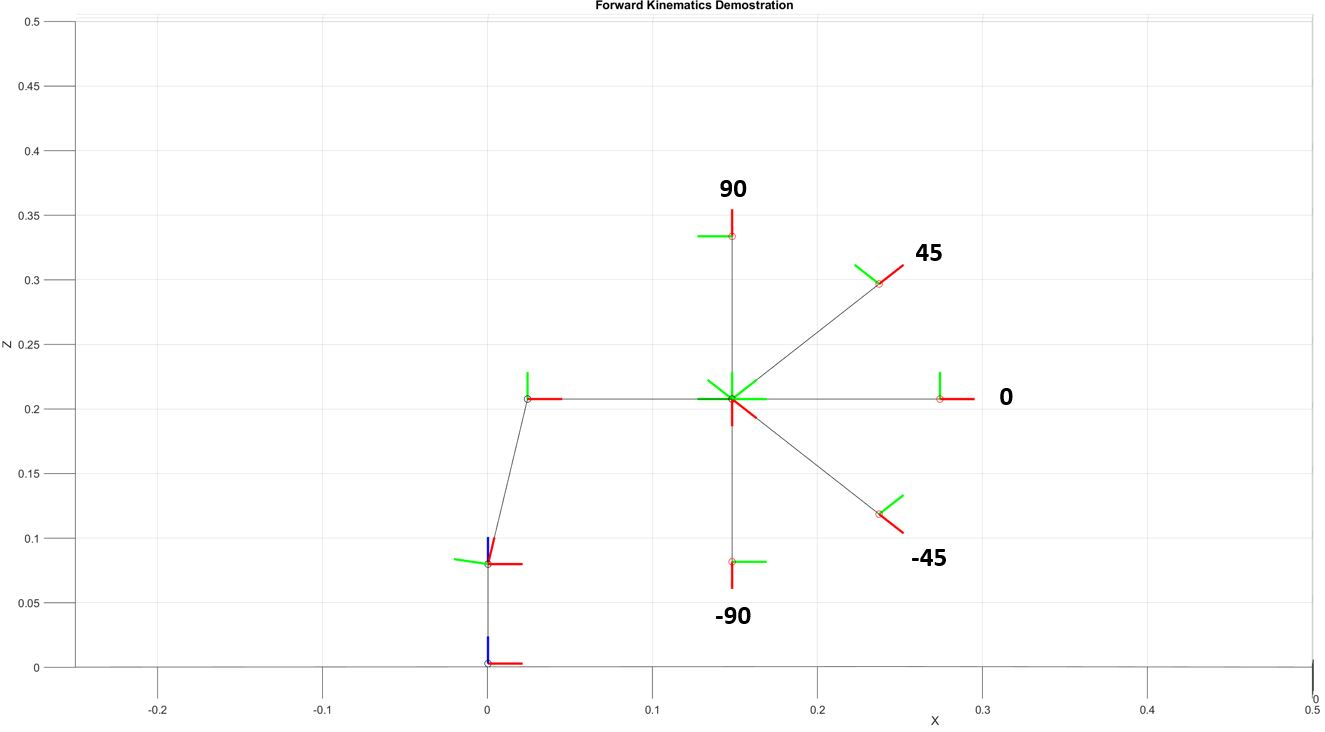
\includegraphics[width=7cm]{theta4.JPG}
    \caption{$\theta_4$ rotation: [$90\degree, 45\degree, 0\degree, -45\degree, -90\degree$]}
  \end{subfigure}
\end{figure}

\subsubsection{Plotting $XYZ$-axis indicators on Co-ordinate Frames}
The $XYZ$-axis indicators of the arm joints are dependent on the current
rotation of the associated joint which, itself, is dependent on the world and any
previous joints related to it i.e. $\theta_i$
where $i$ denotes the specific arm joint. Due to this dependency, the
$xyz$-axis indicators are implemented with a variation of Forward Kinematics where
the $x,y,z$ axis are calculated based on the $\theta_i$ value of the associated
joint. For example, the co-ordinate frame of the \textit{Waist} with rotation $\theta_1$ is calculated
using Forward Kinematics as follows:
{\small
\begin{align*}
  Waist_x &= \begin{bmatrix}
    c(\theta_1) & -s(\theta_1) & 0 & 0.021 \\ 
    s(\theta_1) & c(\theta_1)  & 0 & 0     \\ 
    0 & 0 & 1 & 0 \\ 
    0 & 0 & 0 & 1
  \end{bmatrix} 
  Waist_y &= \begin{bmatrix}
    c(\theta_1) & -s(\theta_1) & 0 & 0 \\ 
    s(\theta_1) & c(\theta_1)  & 0 & 0.021 \\ 
    0 & 0 & 1 & 0 \\ 
    0 & 0 & 0 & 1
  \end{bmatrix} 
  Waist_z &= \begin{bmatrix}
    c(\theta_1) & -s(\theta_1) & 0 & 0 \\ 
    s(\theta_1) & c(\theta_1)  & 0 & 0 \\ 
    0 & 0 & 1 & 0.021 \\ 
    0 & 0 & 0 & 1
  \end{bmatrix} 
\end{align*}
}% 
where the value $0.021$ represents the length of the line of the $xyz$-axis indicator.
\begin{figure}[h]
  \centering
  \begin{subfigure}{.5\textwidth}
    \centering
    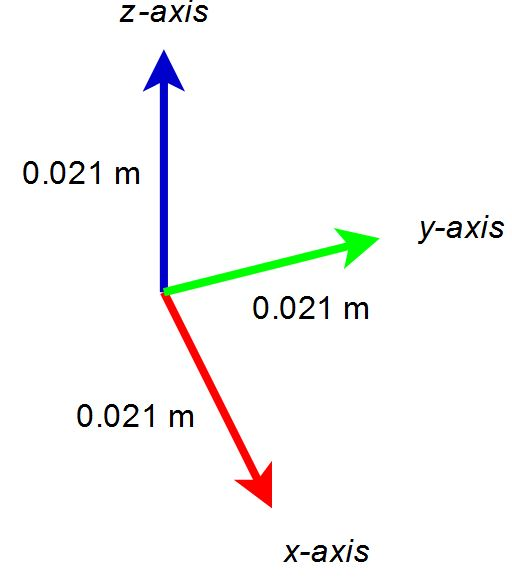
\includegraphics[width=2cm]{frame.JPG}
    \caption{Dimensions of co-ordinate frame}
  \end{subfigure}%
  \begin{subfigure}{.5\textwidth}
    \centering
    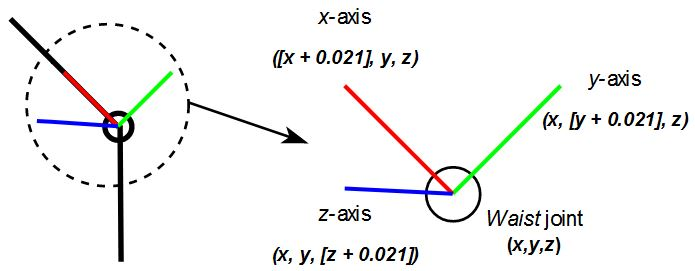
\includegraphics[width=6cm]{joint frames.JPG}
    \caption{Relation of the axis of joint co-ordinate frame to the co-ordinate of the joint}
  \end{subfigure}
\end{figure}

This functionality is implemented as a separate function
\verb+FK_coordinate_frames+ that returns the
$x,y,z$ positions relative to the joint for each of the 5 joints of the arm.

\subsection{Inverse Kinematics}
The inverse kinematics problem for the OpenManipulator-X arm is solved through a
geometric approach that is covered in depth in the Appendix. The following
equations are the solutions to the inverse kinematics problem given co-ordinates
$(x, y, z)$ with robotic arm lengths \cite{CAD_model}: $a_2 = 0.130$, $a_3 = 0.124$ and $a_4 = 0.126$:
\begin{align*}
    \textbf{Waist}: \theta_1 &= \begin{cases} 
        \arctan(\frac{y}{x}) + 180 & x < 0 \text{ and } y > 0 \\ 
        \arctan(\frac{y}{x}) - 180 & x < 0 \text{ and } y < 0 \\
        \arctan(\frac{y}{x}) & \text{otherwise}
    \end{cases} \\
    \textbf{Shoulder}: \theta_2 &= \arctan\left(\frac{\sin(\theta_2)}{\cos(\theta_2)}\right) \\ 
    \textbf{Elbow}: \theta_3 &= -\arccos\left(\frac{r_2^2 + z_2^2 - a_2^2 + a_3^2}{2*a_2*a_3}\right)\\ 
    \textbf{Wrist}: \theta_4 &= \phi - \theta_3 - 90 + \theta_2 
\end{align*}
where:
\begin{itemize}
    \item $\phi$ is the orientation of the end effect that is specified by the user
    \item $r_3 = |\sqrt{x^2 + y^2}|$
    \item $z_3 = z - 0.077$
    \item $z_2 = z_3 - a_4\sin(\phi)$  
    \item $r_2 = r_3 - a_4\cos(\phi)$
    \item $\sin(\theta_2) = \frac{a_2 + a_3*\cos(\theta_3)*r_2 - a_3*\sin(\theta_3)*r_2}{r_2^2 + z_2^2}$
    \item $\cos(\theta_2) = \frac{a_2 + a_3*\cos(\theta_3)*z_2 - a_3*\sin(\theta_3)*z_2}{r_2^2 + z_2^2}$
\end{itemize}

Further conversions are required to convert the angles outputted from inverse
kinematics to the angles compatible with the openManipulator-X arm servos as
defined in the \verb+Appendix: Task 1: Inverse Kinematics+.

\subsubsection{Inverse Kinematics Simulation: Tracing a square on each cartesian plane}

To test the functionality of the inverse kinematic solver, the robotic arm draws
a cube in 3D space. The process is summarised as follows: 
\begin{itemize}
  \item Start and end co-ordinate of each line of the cube is specified. Using
  matlab \verb+linspace+, the co-ordinates of the points between the
  start and end points are generated 
  \item These sets of co-ordinates are concatenated together in the order the
  arm traverses over them 
  \item The combined set is iterated in a FOR loop, each co-ordinate fed into
  the \verb+IK+ function that specifies the joint angles required to achieve
  the specified co-ordinate
\end{itemize}
\begin{figure}[h]
    \centering
    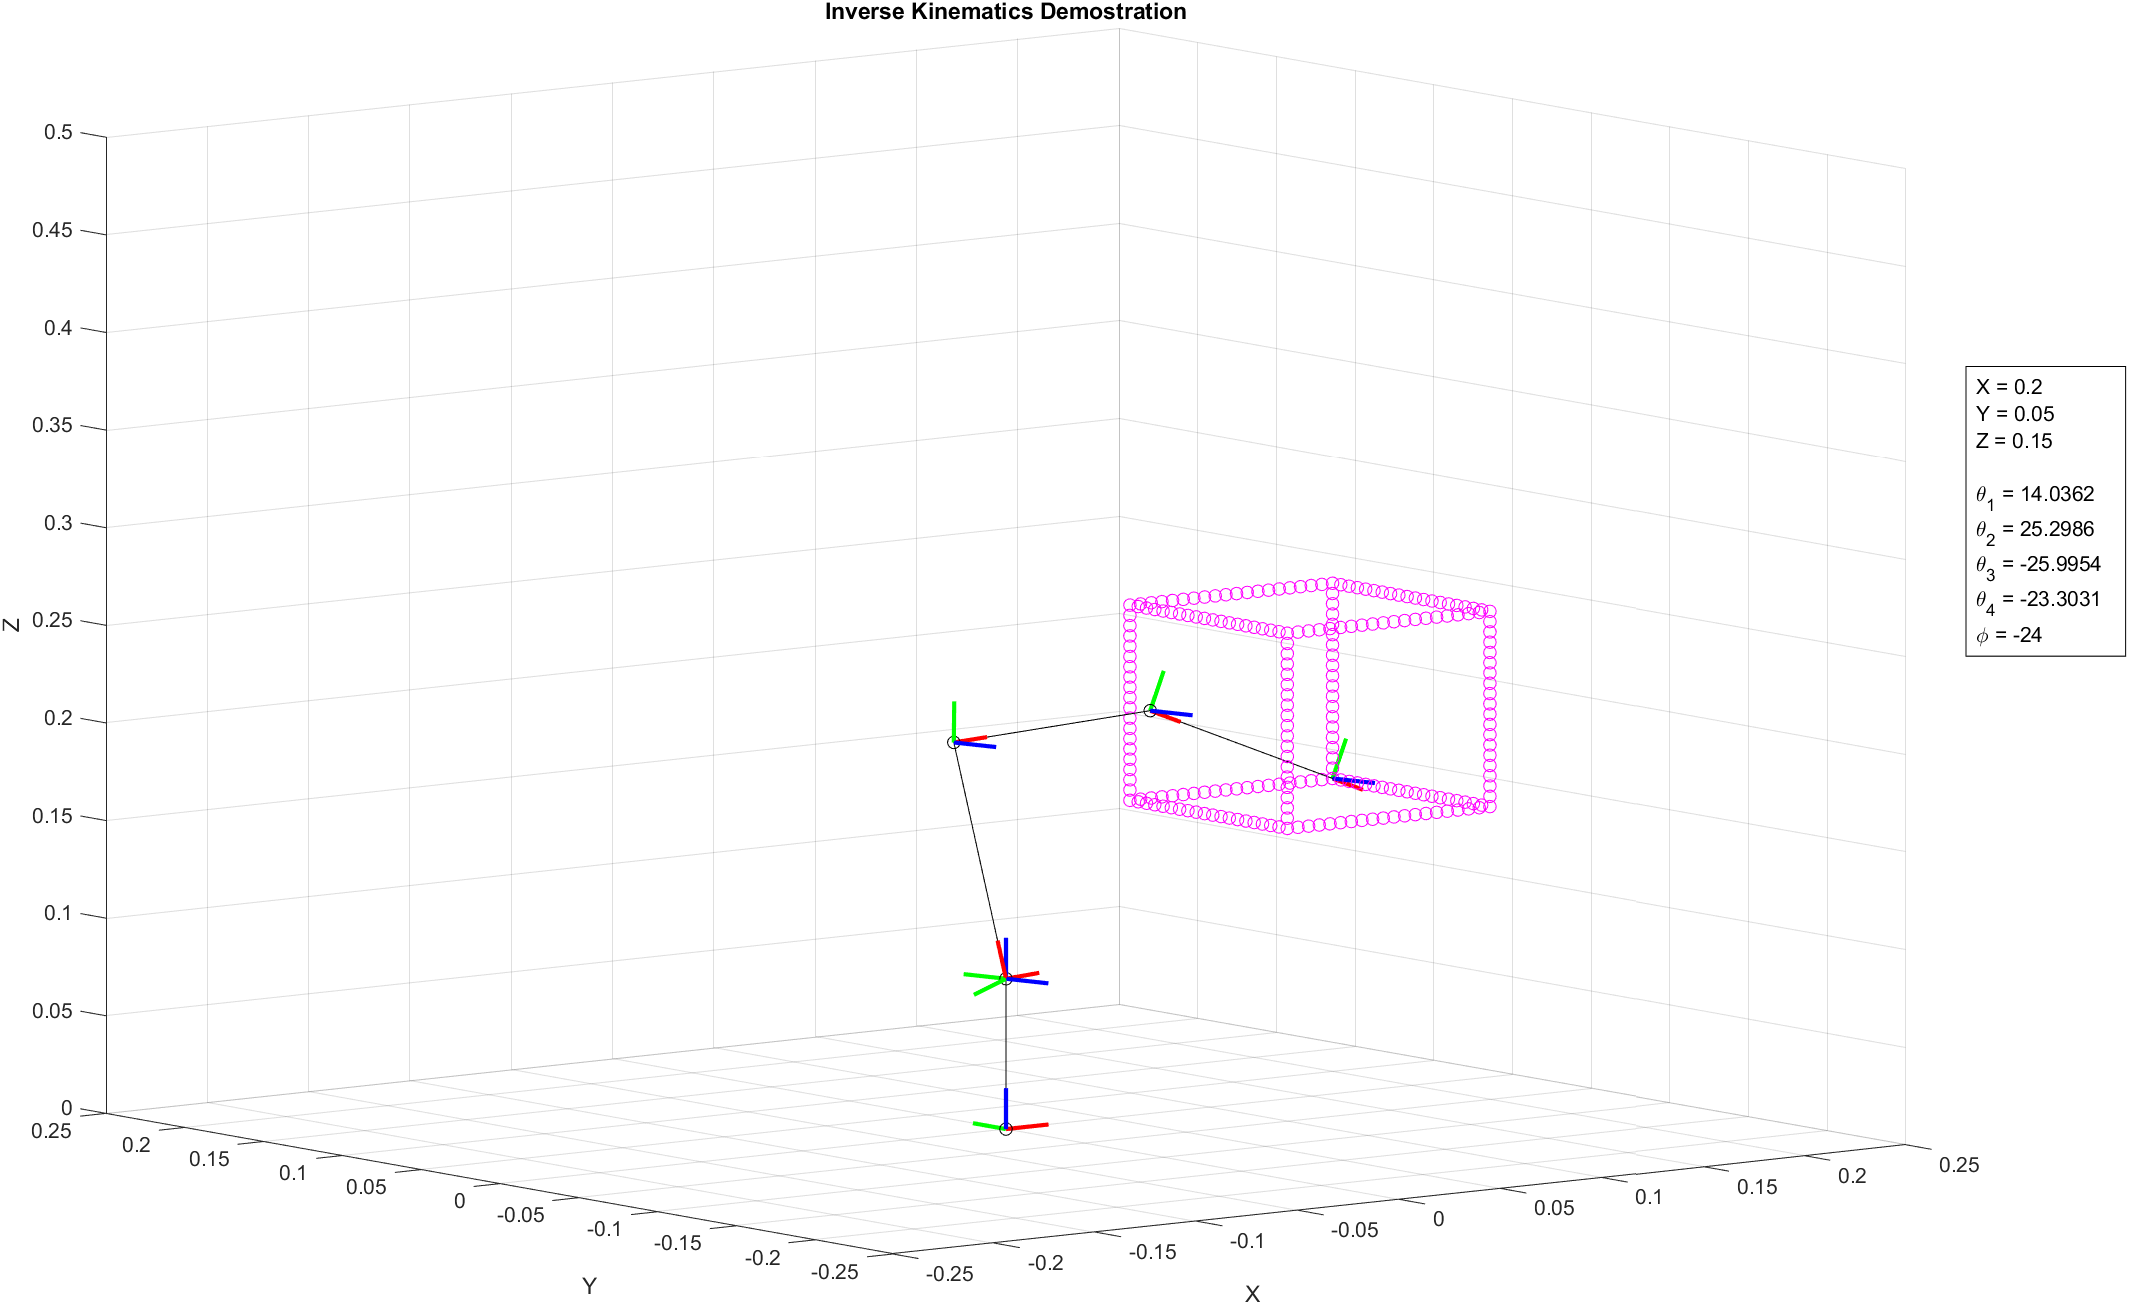
\includegraphics[width=7cm]{6}
    \hspace{1cm}
    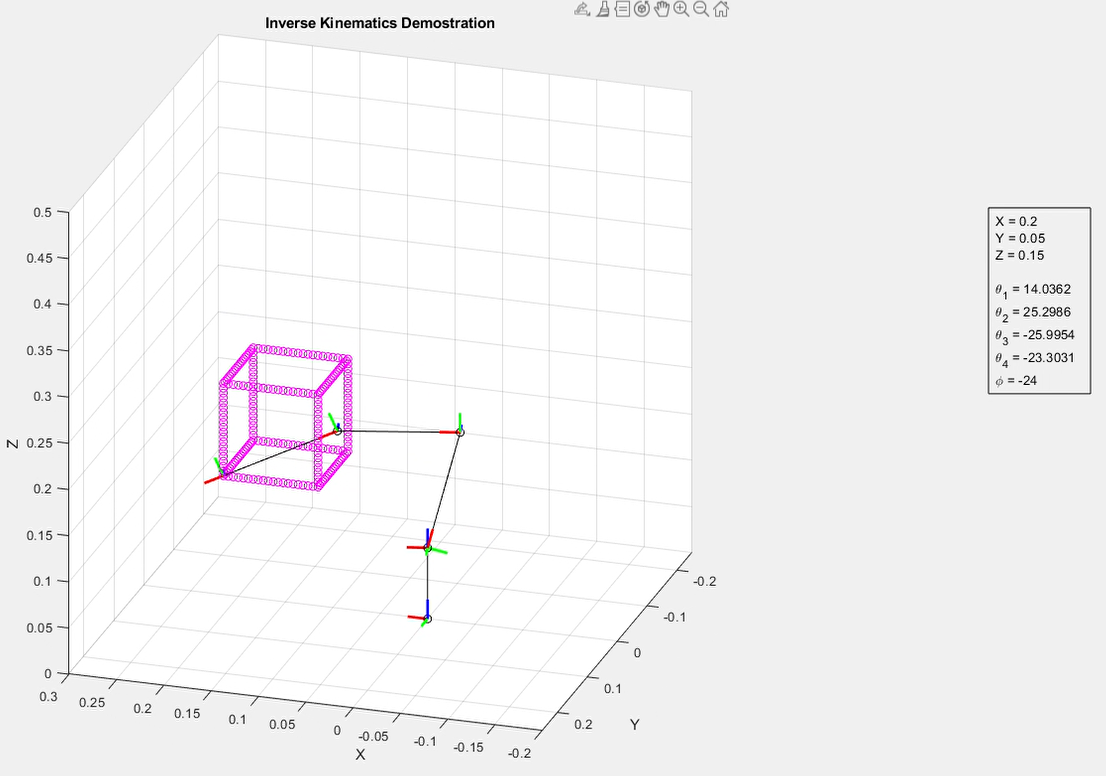
\includegraphics[width=7cm]{7}
\end{figure}

\vfill
\pagebreak

%%%%%%%%%%%%%%%%%%%%%%%%%%%%%%%%%%%%%%%%%%%%%%%%%%%%%%%%%%%%%%%%%%%%%%%%%%%%%%%%%%%%%%%%%%%%%%%%%%%%%%%%%%
\section{Task 2 - Pick and Place Cubes}

Task 2 was broken down into several modular components that enabled the team to
divide the work and tackle it separately. 
\begin{enumerate}
  \item \textbf{Picking up and dropping function}
  
  Given the $(x,y,z)$ co-ordinates of the cubes, the Inverse Kinematics solver
  will calculate the servo angles required to reach that co-ordinate. In the
  Inverse Kinematics solver, the team has added multiple checks that ensures
  only reachable co-ordinates are allowed to be fed into the arm. 
  
  For picking and dropping tasks, the team made the design decision to only pick up and drop cubes from
  the top ($\phi = -90 \degree $) if it is reachable. Otherwise if the cube is too far then the
  robot would pick and drop cubes from the middle ($\phi = 0 \degree $) as this is able to
  extend the range by a tiny amount. However picking up at ($\phi =  0 \degree $) has to be
  shifted up as picking up from the middle causes the cube holders to be gripped.
  Some ranges of close range picking up/dropping can't be achieved with
  ($\phi = 0 \degree $) thus a cube is picked up/dropped at ($\phi = -90 \degree
  $) for close ranges. However if a cube is picked from far range ($\phi = 0\degree $) and dropped at close range
  ($\phi = -90 \degree $) or vice versa the appropriate transformations would have to be taken
  into account due to the cube being shifted up when being picked by ($\phi = 0\degree $).

  For picking and dropping tasks, the team made the design decision to only pick
  up and drop cubes from the top $(\phi = -90)$. This was due to the fact that
  picking/dropping from horizontal direction $(\phi=0)$ would cause the gripper
  extrusions to hit the cube holders and increasing the height at which the
  gripper grips the cube would result in a very loose grip. 
  
  \item \textbf{Rotate cube function}
  
  Rotating cubes are divided into two types: Rotating forward and rotating
  backward. The key to completing this task was understanding that $\phi$
  determines the final orientation of the end-effector (\textit{Gripper}). With
  that, a cube can be rotated by picking it up with $\phi = 0$ and dropping it in
  the same place with $\phi = -90$, and vice versa for the opposite direction. 
\end{enumerate}
\begin{figure}[h]
  \centering
  \begin{subfigure}{.5\textwidth}
    \centering
    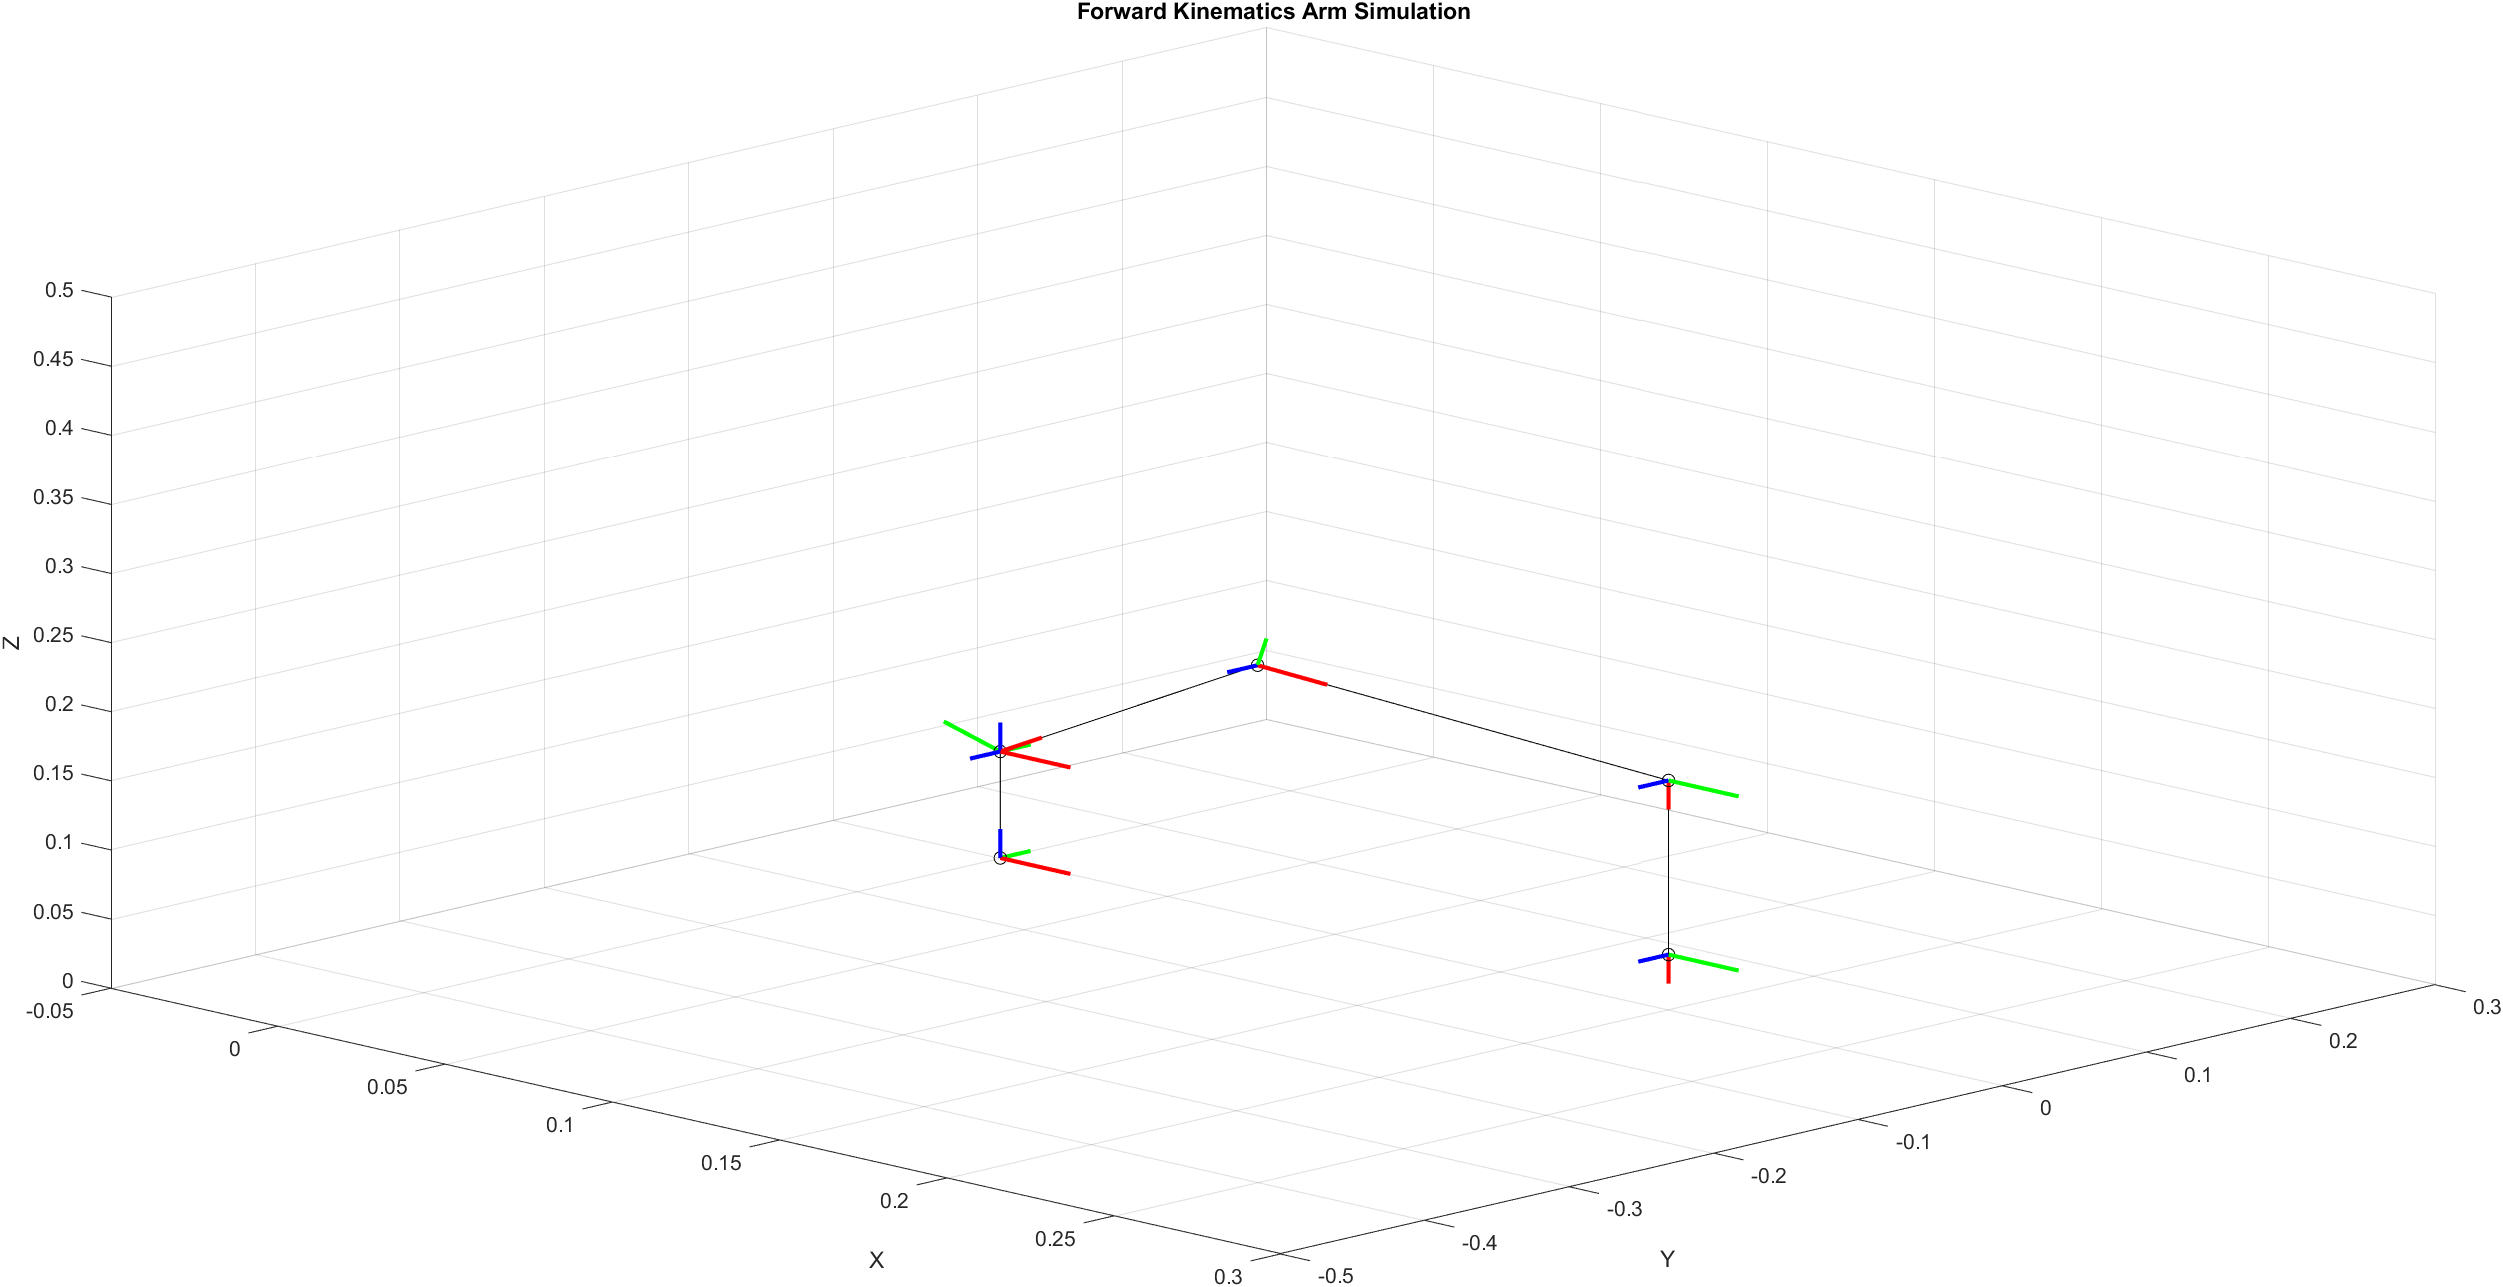
\includegraphics[width=7cm]{1}
    \caption{Picking up cube: $\phi = -90\degree$}
  \end{subfigure}%
  \begin{subfigure}{.5\textwidth}
    \centering
    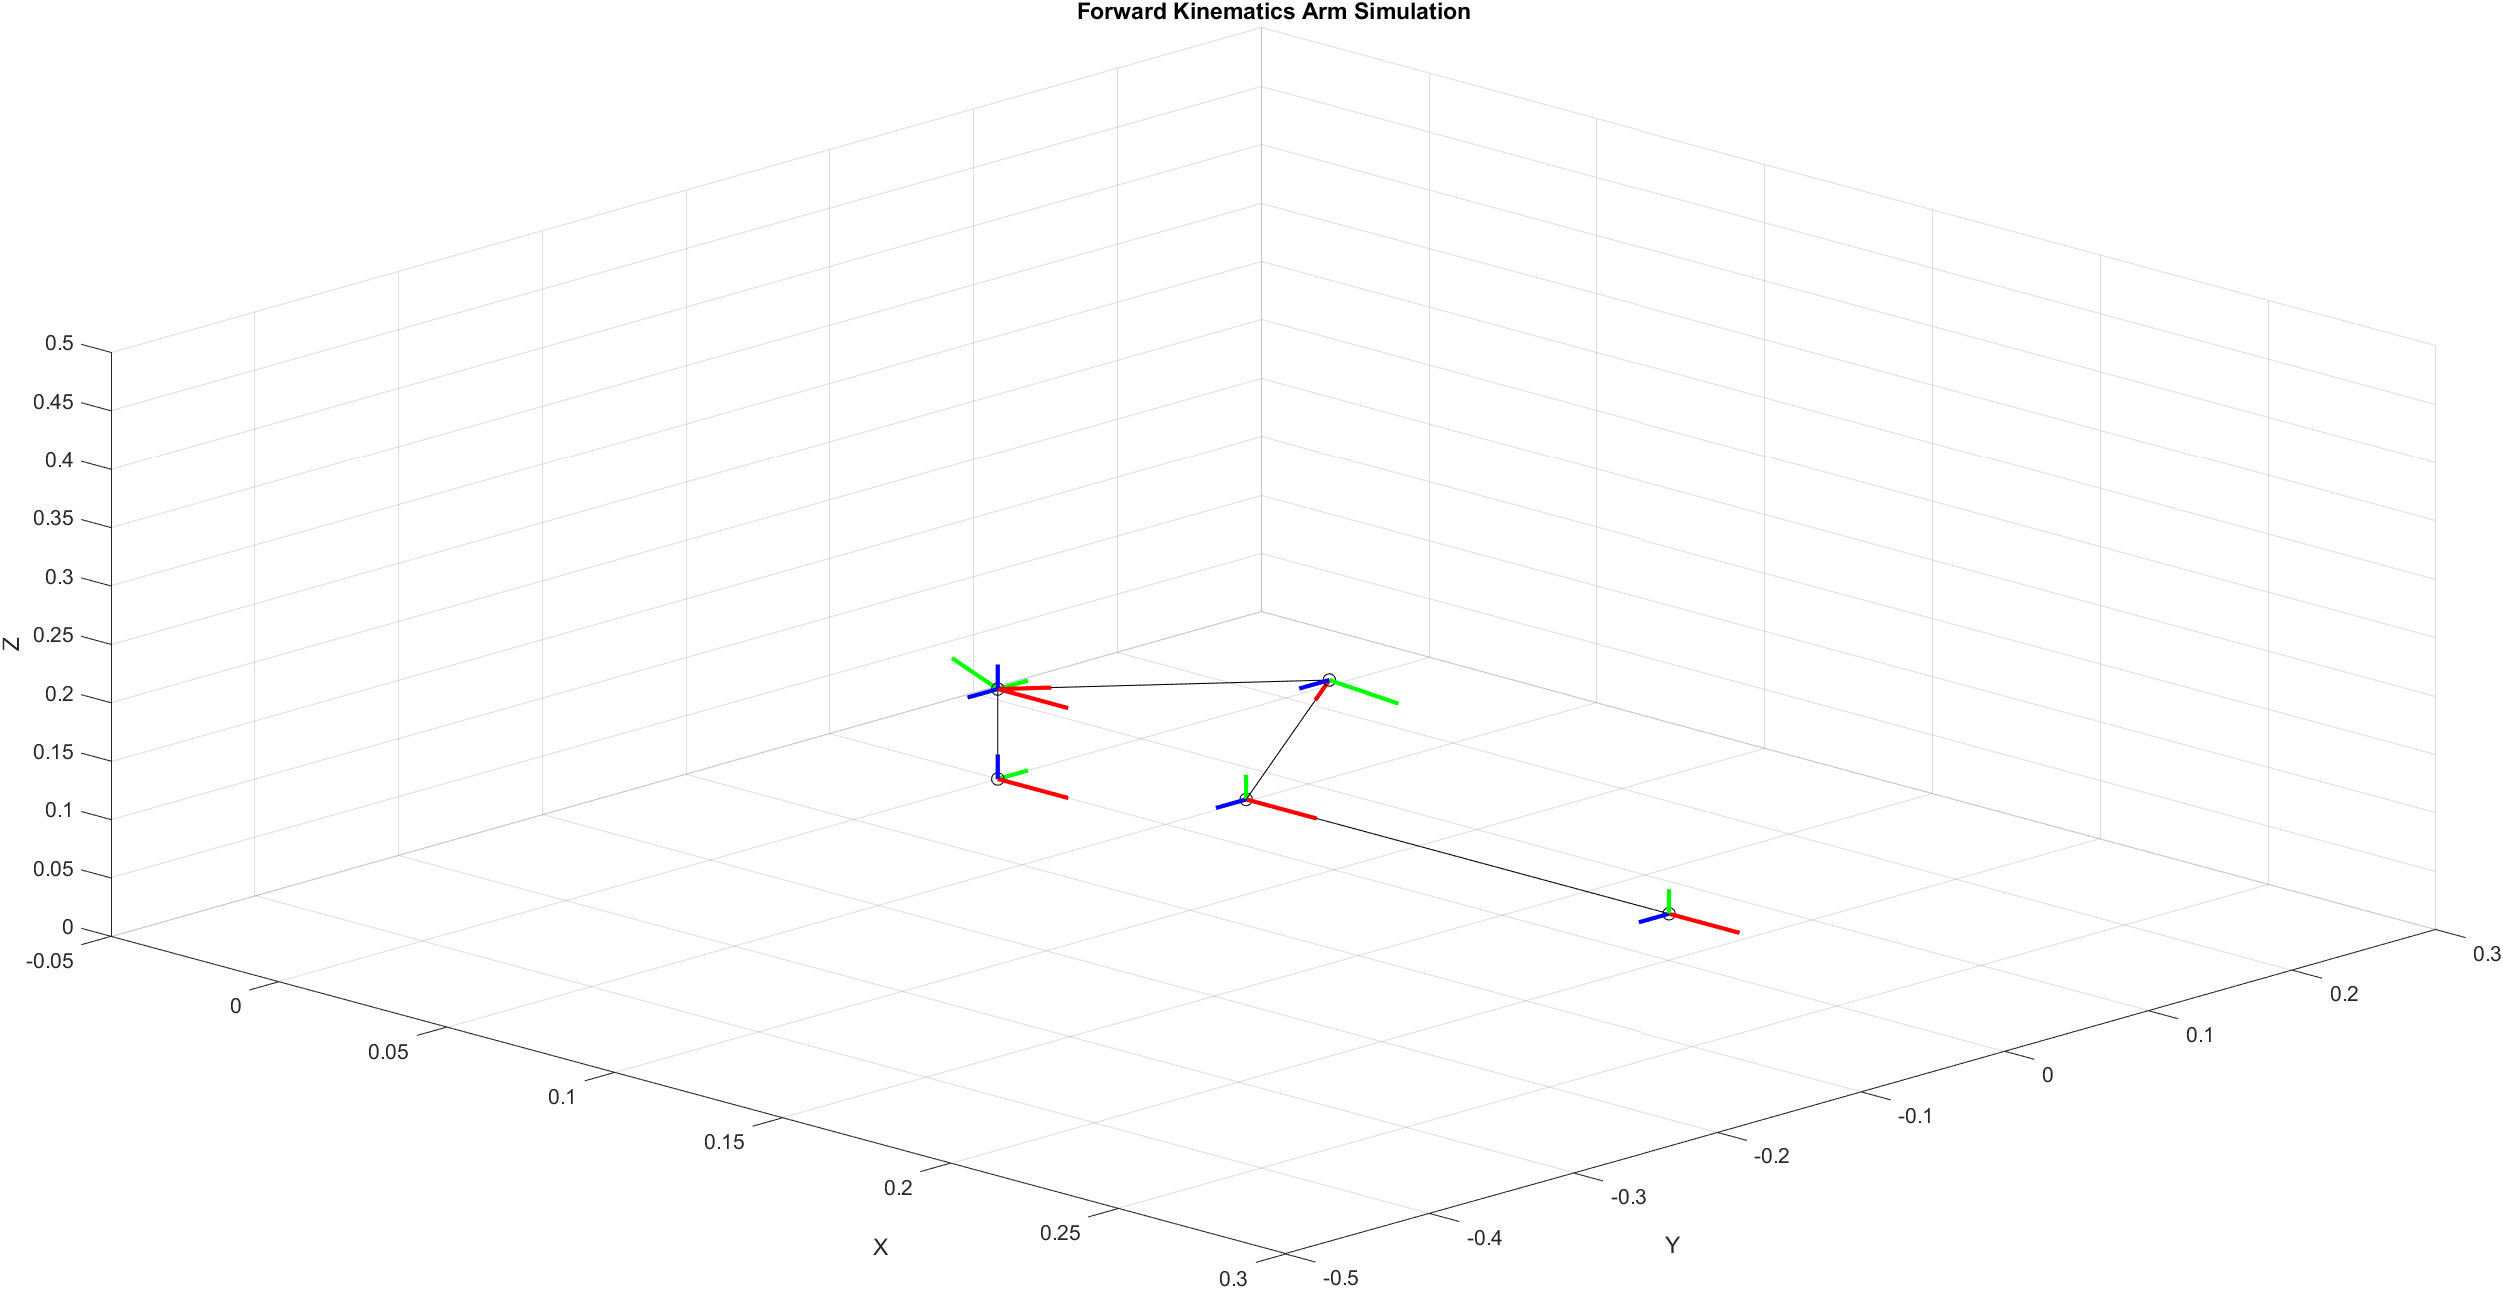
\includegraphics[width=7cm]{2}
    \caption{Dropping cube: $\phi = 0\degree$}
  \end{subfigure}
  \caption{Depiction of backward rotation}
\end{figure}

\begin{enumerate}
  \setcounter{enumi}{2}
  \item \textbf{Stacking cube function}
  
  The action of stacking is a combination of rotating and picking
  up/dropping cubes. Therefore, the arm is designed to first rotate all the cubes
  then proceed to picking up and drop the cubes at a height increasingly $0.025m$ higher to
  account for the height of the already stacked cubes. 
  
  \item \textbf{Co-ordinates of sockets on the acrylic board}
  
  With the OOP approach, the co-ordinates of every socket on the
  acrylic board could be stored as three matrices representing the $x, y$ and $z$
  values of a specific socket. To obtain the co-ordinates of a socket, the row and
  column of the desired socket is specified and the function returns the $(x,y,z)$
  co-ordinates for the associated row and column.  

  \item \textbf{Linear interpolation}
  
  Basic linear interpolation is implemented to prevent the arm moving in an
  undesired way. This is important for picking/dropping and rotating cubes where,
  without linear interpolation, could approach the cube holders from the sides
  and hit the protruded edges of the cube holders. For stacking, the behaviour
  of the arm for a particular action would be unpredictable and acidentally hit
  the stacked cubes. 

  \begin{figure}[h]
      \centering
      \includegraphics[width=7cm]{Linear}
      \caption{Illustration of arm going down to pick up a cube with linear interpolation}
  \end{figure}

  Linear interpolation affects the action of moving down and moving up
  from cube co-ordinates. For any particular cube co-ordinate, the arm would first move to directly
  that co-ordinate with a $z$-offset of at least $+0.030m$. Once there, there
  are 3 waypoints, each with a decreasing $z$-offset where the last waypoint is
  the co-ordinate to pick up/drop off the cube. The reverse happens for the
  arm moving back up.

  For transit i.e. when the arm picks up a cube and moving to another
  co-ordinate to drop off the cube, no linear interpolation is required. The arm
  automatically determines the best way to reach the drop-off co-ordinate with a
  $z$-offset of at least $+0.030m$. This approach was taken to ensure the
  smoothest possible movement without implementing velocity control. 
  
  To further ensure smooth motion, we investigated the concept of writing the
  next waypoint to the servo motors when travelled a certain distance between
  the two waypoints it is currently trying to get to. This is due to the robot
  having it's own interpolation when in position control mode thus resulting in
  a stuttery movement when using linear interpolation naively. Provided the next
  waypoint is not the final one, the current distance travelled between the two
  waypoints (starting and finishing) is calculated. Using this, a percentage of
  how much the robot has travelled between the two waypoints is also calculated
  and when the robot has travelled a certain proportion of the overall distance
  the next waypoint will be written. This is because the robot's stuttering is
  due to the robot slowing down before reaching it's waypoint (from it's own
  interpolation) thus if the robots waypoint is overwritten when it still has
  not slowed down, this results in a smoother motion.
 
  \item \textbf{Calibration mechanisms}
  
  There is a certain amount of uncertainty with the robotic arm and, with the
  team working with different arms each time, a system had to be
  implement to be able to streamline the calibration of the arm. Each function
  related to manipulation such as \verb+move_cube_coord+ has two calibration
  parameters: 
  \begin{figure}[h]
      \centering
      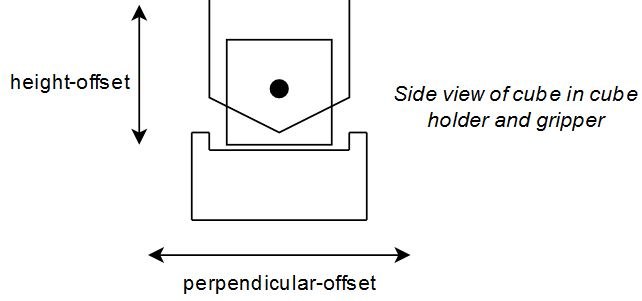
\includegraphics[width=8cm]{side view.JPG}
  \end{figure}
  \begin{itemize}
    \item \verb+height_offset+: Increases/decreases the $z$ co-ordinate  
    \item \verb+perpendicular_offset+: Increases and decreases the perpendicular
    distance e.g. dropping the cube a bit more forward or bit more backward
  \end{itemize}
\end{enumerate}

%%%%%%%%%%%%%%%%%%%%%%%%%%%%%%%%%%%%%%%%%%%%%%%%%%%%%%%%%%%%%%%%%%%%%%%%%%%%%%%%%%%%%%%%%%%%%%%%%%%%%%%%%%
\section{Task 3 - Trajectory Following (Drawing)}

Task 3 is split into two components with sub-components: 
\begin{itemize}
  \item Pick up a pen and placing it back 
  \item Drawing a given pattern composed of:
  \begin{itemize}
    \item Three straight lines in different directions such as horizontal, vertical, and diagonal
    \item A circle with a given radius, center point and degree of rotation 
  \end{itemize}
\end{itemize}

The team's approach to solving Task 3 is summarised as follows:
\begin{enumerate}
  \item A visualiser i.e. plotting function to see the pattern a set of
  generated co-ordinates would create 
  \item Modifying the DH table. The modified DH table can be seen in
  \verb+Appendix: Task 2 and 3 modified+ \verb+DH Table+
  \item Designing the pen grippers:
  
  When designing the pen gripper, two main factors had to be taken into account:
  \begin{itemize}
    \item Ensure the pen wouldn't slip out as the robot applies pressure on it when drawing
    \item Ensure the stability of the pen to obtain the straightest lines possible when drawing
  \end{itemize}

  It was noted that the pen provided had an outline that slightly decreases
  towards the tip. The pen gripper surface accounts for that decrease in
  gradient to ensure the tightest grip possible. The CAD model can be accessed 
  under \verb+Appendix: Task 2 and 3 CAD models+ 

  \item Implementing global parameters that would generalise the drawing process
  allow different patterns to be created with minimal changes 
  \item Concatenating all the generated co-ordinates into a large array,
  converting to angles through Inverse Kinematics and feeding all the angles to the robot 
\end{enumerate}

For drawing, different approaches were used for drawing lines and circles:
\begin{itemize}
  \item \textbf{Straight lines}: Having specified the start and end
  co-ordinates, Matlab's built-in colon operator generates evenly spaced vectors
  of $i$ increments. This allowed the team to control how many way-points are
  created. With the horizontal line, the $x$-axis changes while the $y$-axis
  remains the same. The reverse occurs for vertical lines. For diagonal lines, it
  is drawn by considering it as a function $y=x$ where $x$ and $y$ increments
  simultaneously. The orientation of the diagonal can be chosen by setting
  accordingly the start and end point as well as modifying the increment to a
  negative or positive slope depending on the wanted orientation of the
  diagonal.  

  Note that the commonly thought $x$ and $y$ axis are inverted due to our frame
  choice.
\end{itemize}
\begin{itemize}
  \item \textbf{Circles}: Circles are drawn using a derivation of the classical circle
  equation:
  \begin{gather*}
    x = \text{radius} * \cos(\theta) + \text{center point x} \\
    y = \text{radius} * \sin(\theta) + \text{center point y} \\
    x^2 + y^2 = r^2
  \end{gather*}

  From the inputted degree of the circle, the equivalent radian value is calculated
  and $\theta$ values to reach it from the starting point on the 
  circle are obtained. The \verb+linspace+ function was used to increment theta and
  define how many points are fed to the robot. Using the circle equation and
  considering the circle center and radius, we calculate the corresponding $x$ and
  $y$ coordinates for each theta angles. This process ensures a well-defined and
  precise circle.  
\end{itemize}

% CAD design 
%%%%%%%%%%%%%%%%%%%%%%%%%%%%%%%%%%%%%%%%%%%%%%%%%%%%%%%%%%%%%%%%%%%%%%%%%%%%%%%%%%%%%%%%%%%%%%%%%%%%%%%%%%
\section{Task 4 - Musical instruments}

For Task 4, the team chose to perform a musical piece using drums and a
xylophone. Music is complex to the robotic arm in the sense that the timings at
which the notes are hit must be approximately correct. This meant that the
speeds of the arm servos are all different and changes continuously throughout
the musical performance. If any servos was wrongly calibrated or the arm does
not hit the instruments fast enough, the musical piece would immediately sound
wrong. This challenge was interesting to the team and we
felt that it was a suitable task to show the skills we learnt throughout the
course of this module and through working with the robotic arm. 

% TODO: Describing task

This task was broken down into the following steps:
\begin{enumerate}
  \item Designing the gripper to hold the xylophone stick 
  
  For the xylophone gripper, a similar approach to the pen holder was taken. As the xylophone's
  stick radius is uniform across its whole length the designed grippers were
  slightly loose on some movements. We adapted by wrapping the stick with a
  rubbery material which fixed our issue. The CAD model can be accessed under
  \verb+Appendix: Task 2 and 3 CAD models+ 
  
  \item Placing musical instruments in reachable range and using forward
  kinematics to note down the coordinates of drums and xylophone tone bars
  
  To account for the change in gripper design, the original DH table is
  modified. The modified DH table can be seen in the \verb+Appendix: Task 2 and 3 modified DH Table+

  \item Creating functions to hit drums and specified tone bars 
  
  Functions were created that handled the actions of hitting drums and tone
  bars. With the OOP approach taken by the team, many pieces of code could be
  re-used and slightly adjusted for this particular task. This modular approach
  code allowed the team to easily identify and finely adjust factors on the fly such as
  velocity and acceleration. 
  
  \item Calibrating the hit action and combining hits to produce a recognisable piece of music 
  
  Calibrating the hit action involved 3 tasks: Timing the hit properly and
  hitting the xylophone with the right power and accuracy. 
  \begin{itemize}
    \item Accuracy can be achieved by simply modifying the DH table to account
    for the difference in gripper length and also calibrating taking into
    account the weight of the xylophone stick. 
    \item Timing can be controlled by 2 parameters, the height in which the
    robot gripper would hover above the xylophone and the speed of some motors
    (more specifically motors 11 and 14). Decreasing the height means the robot
    would need to travel less distance in order to hit a key on the xylophone.
    Incresing the motor speed means each hit will take less time as the robot
    will get to it's destination faster. The 2 most important motors to modify
    is motor 11 ($\theta_1$) and motor 14 ($\theta_4$). Throughout a song, both
    parameters are modified to either increase or decrease the tempo. A tradeoff
    of both are important to ensure appropriate power when hitting a key is also
    satisfied. 
    \item Power is simply controlled by the motor speed servo motor 14 ($\theta_4$).
    However power is also linked with timing (when power is decreased, the travel
    time increases) thus the appropriate height has to be modified accordingly 
  \end{itemize}
\end{enumerate}

%%%%%%%%%%%%%%%%%%%%%%%%%%%%%%%%%%%%%%%%%%%%%%%%%%%%%%%%%%%%%%%%%%%%%%%%%%%%%%%%%%%%%%%%%%%%%%%%%%%%%%%%%%
\pagebreak
\section{Appendix}
\subsection{Task 1: Forward Kinematics}

Note the dimensions \cite{CAD_model}: 
\begin{itemize}
  \item Height offset from base to \textit{Waist} joint: 0.077 m
  \item Length of hypotenus from \textit{Waist} joint to \textit{Elbow} joint:
  0.130 m 
  \item Length from \textit{Elbow} joint to \textit{Wrist} joint: 0.124 m 
  \item Length from \textit{Wrist} joint to \textit{Gripper} end effector: 0.126 m
\end{itemize}

Forward kinematics matrices:
\begin{align*}
  T^{\text{Base}}_{\text{Waist}} &= \begin{bmatrix}
    \cos(\theta_1) & -\sin(\theta_1) & 0 & 0 \\
    \sin(\theta_1) & \cos(\theta_1) & 0 & 0 \\ 
    0 & 0 & 1 & 0.077 \\
    0 & 0 & 0 & 1
    \end{bmatrix} \\ 
  T^{\text{Waist}}_{\text{Shoulder}} &= \begin{bmatrix}
    \cos(\theta_2 + 10.62) & -\sin(\theta_2 + 10.62) & 0 & 0 \\
    0 & 0 & -1 & 0 \\ 
    \sin(\theta_2 + 10.62) & \cos(\theta_2 + 10.62) & 0 & 0 \\
    0 & 0 & 0 & 1
    \end{bmatrix} \\
  T^{\text{Shoulder}}_{\text{Elbow}} &= \begin{bmatrix}
    \cos(\theta_3 - 10.62) & -\sin(\theta_3 - 10.62) & 0 & 0.130 \\
    \sin(\theta_3 - 10.62) & \cos(\theta_3 - 10.62) & 0 & 0 \\ 
    0 & 0 & 1 & 0 \\
    0 & 0 & 0 & 1
    \end{bmatrix} \\
  T^{\text{Elbow}}_{\text{Wrist}} &= \begin{bmatrix}
    \cos(\theta_4) & -\sin(\theta_4) & 0 & 0.124 \\
    \sin(\theta_4) & \cos(\theta_4) & 0 & 0 \\ 
    0 & 0 & 1 & 0 \\
    0 & 0 & 0 & 1 
    \end{bmatrix} \\
  T^{\text{Wrist}}_{\text{Gripper (end-effector)}} &= \begin{bmatrix}
    1 & 0 & 0 & 0.126 \\
    0 & 0 & 0 & 0 \\ 
    0 & 0 & 1 & 0 \\
    0 & 0 & 0 & 1 
    \end{bmatrix} \\  
\end{align*}

\subsection{Task 1: Inverse Kinematics}

The process to solve for the Inverse Kinematics equations given a set of
co-ordinates $(x,y,z)$ is split into two sections: $x-y$ domain and $r-z$
domain.

Note the dimensions of the robotic arm \cite{CAD_model}: $a_2 = 0.130, a_3 = 0.124, a_4 = 0.126$


\subsubsection{$x-y$ domain}
The angle for the \textit{Waist} joint, given co-ordinates $(x, y, z)$ can be calculated as:
$$
  \theta_1 = \arctan \left(\frac{y}{x}\right)
$$

Note that the \textit{Waist} joint rotation range is between $-180\degree$ to
$180\degree$ with the middle point being $0\degree$. Therefore it is important
to ensure that the angles are within that range for any combination of $p_x$ and
$p_y$.
$$
\theta_1 = \begin{cases} 
  \arctan(\frac{y}{x}) + 180 & x < 0 \text{ and } y > 0 \\ 
  \arctan(\frac{y}{x}) - 180 & x < 0 \text{ and } y < 0 \\
  \arctan(\frac{y}{x}) & \text{otherwise}
\end{cases}
$$

\subsubsection{$r-z$ domain}

Angles for the \textit{Shoulder} ($\theta_2$), \textit{Elbow} ($\theta_3$) and
\textit{Wrist} ($\theta_4$) are solved in the $r-z$ domain. The $r-z$ domain is
a simplified view of the 3D space ($x,y,z$) where the $x$ and $y$ axis are
merged using the Pythagorean equation 
$$
  r = \sqrt{x^2 + y^2}
$$
to define the $r$ axis as shown in the image Figure 4(a).
\begin{figure}[h]
  \centering
  \begin{subfigure}{.5\textwidth}
    \centering
    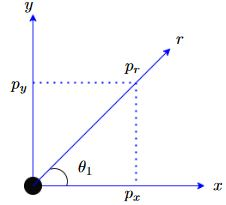
\includegraphics[width=4cm]{r.JPG}
    \caption{$r$-axis a result of merging the $x$ and $y$ axis}
  \end{subfigure}%
  \begin{subfigure}{.5\textwidth}
    \centering
    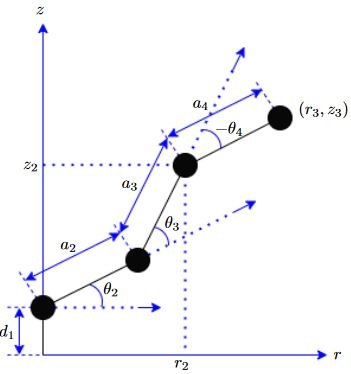
\includegraphics[width=5cm]{arm r domain.JPG}
    \caption{Robotic arm projected onto the $r-z$ domain}
  \end{subfigure}
  \caption{\cite{Coordinate_frame}}
\end{figure}

In order to solve the inverse kinematic equations, the variable term $\phi$ has
to be defined which, in this case, is defined as the sum of the angles
$$
  \phi = \theta_2 + \theta_3 + \theta_4
$$

The co-ordinates $(r_3, z_3)$ could easily be calculated given co-ordinates $(x,
y, z)$:
\begin{gather*}
  r_3 = \sqrt{x^2 + y^2} \\ 
  z_3 = z - d_1
\end{gather*}
where $d_1 = 0.077$ m

With $(r_3, r_3)$ and $\phi$, the co-ordinates $(r_2, z_2)$ can be found:
\begin{gather*}
  r_2 = r_3 - a_4 \cos(\phi) \\ 
  z_2 = z_3 - a_4 \sin(\phi)
\end{gather*}

The \textit{Elbow} joint angle can therefore be defined as:
\begin{gather*}
  \theta_3 = \pm \arccos \left( \frac{r_2^2 + z_2^2 - (a_2^2 + a_3^2)}{2 a_2 a_3} \right)
\end{gather*}

With $\theta_3$, co-ordinates $(r_2, z_2)$ can be alternatively defined using
$\theta_2$ and $\theta_3$:
\begin{gather*}
  r_2 = a_2 \cos(\theta_2) + a_3\cos(\theta_2 + \theta_3) \\ 
  z_2 = a_2 \sin(\theta_2) + a_3\sin(\theta_2 + \theta_3)
\end{gather*}

Expanding with Ptolemy's identities:
\begin{gather*}
  r_2 = \cos(\theta_2)\left(a_2 + a_3\cos(\theta_3)\right) - a_3\sin(\theta_2)\sin(\theta_3) \\ 
  z_2 = a_3\cos(\theta_2)sin(\theta_3) + \sin(\theta_2)(a_2 + a_3\cos(\theta_3))
\end{gather*}

By recognising the hypotenus, adjacent and opposite of the triangle subtended by
$\theta_2$:
\begin{gather*}
  \cos(\theta_2) = \frac{r_2(a_2 + a_3 \cos(\theta_3)) + z_2(a_3 \sin(\theta_3))}{r_2^2 + z_2^2} \\ 
  \sin(\theta_2) = \frac{z_2(a_2 + a_3 \cos(\theta_3)) + r_2(a_3 \sin(\theta_3))}{r_2^2 + z_2^2} 
\end{gather*}

Thus the angle $\theta_2$ can be found:
\begin{gather*}
  \theta_2 = \arctan \left(\frac{\sin(\theta_2)}{\cos(\theta_2)}\right)
\end{gather*}

By using the relation of $\phi$, $\theta_2$, $\theta_3$, $\theta_4$ can be
found:
$$
  \theta_4 = \phi - \theta_2 - \theta_3
$$

As mentioned previously, further conversion is before it is fed into the servo
motors. The conversion equations are as follows:
\begin{align*}
  \theta_{1_{servo}} &= 180\degree - \theta_{1_{IK}} \\ 
  \theta_{2_{servo}} &= 180\degree + (\theta_{2_{IK}} - 10.62\degree) \\ 
  \theta_{3_{servo}} &= 180\degree + (-\theta_{3_{IK}} - 79.38\degree) \\ 
  \theta_{4_{servo}} &= 180\degree - \theta_{4_{IK}}
\end{align*}

\subsection{Unity simulation}

Due to the limited number of arms and initial uncertainty in lab times, the team
wanted to mitigate any negative impacts that could arise. With the simulation
tasks in Task 1, one of the team members with game development experience
proposed a virtualised environment where we can interact with the arm with
accurate dimensions and physics. 

As a result, alongside simulating in Matlab, the team created a custom Unity-based
simulation that allowed us to further visualise how the arm would look given
specific angles and to check whether the arm would grip the cube or not. This
allowed us to verify if our forward kinematics and inverse kinematics solvers
are working correctly. 
\begin{figure}[h]
    \centering
    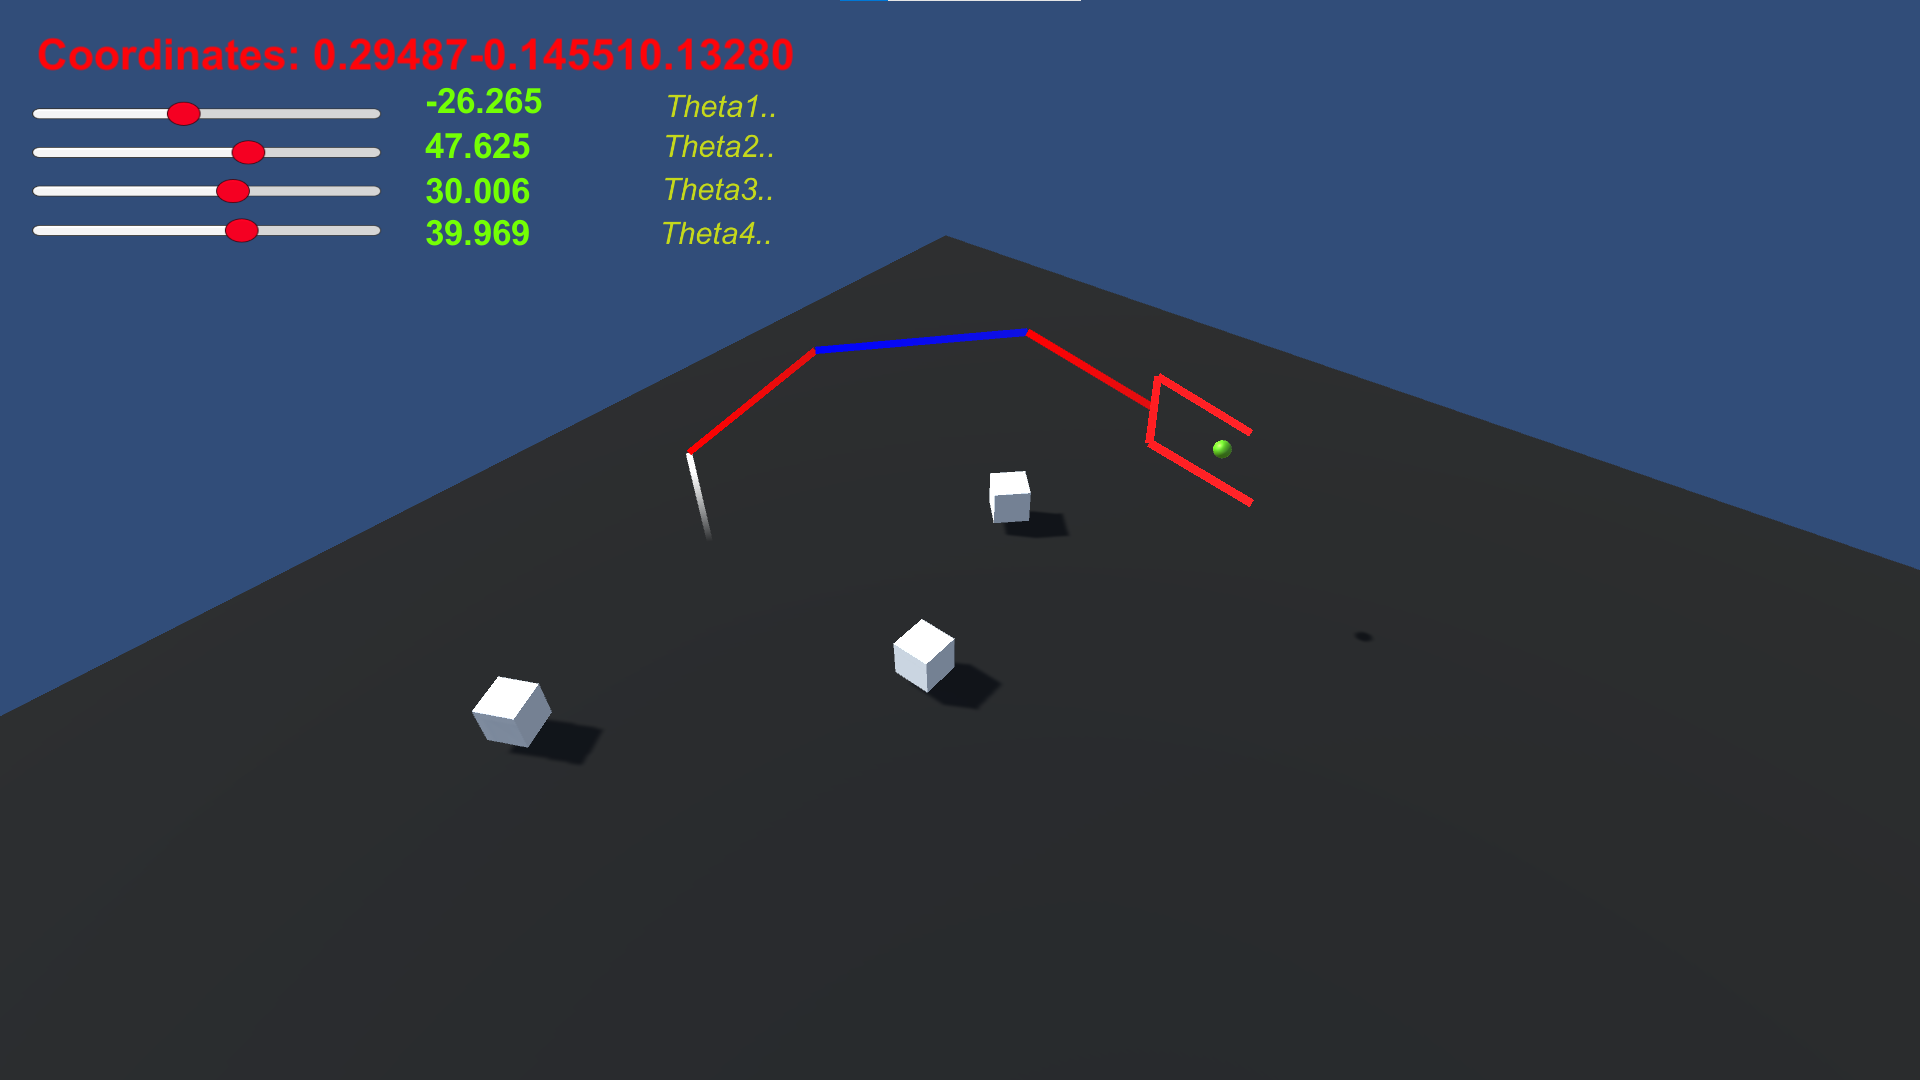
\includegraphics[width=6.5cm]{moving.png}
    \caption{Virtual environment with to-scale robotic arm and cubes. Cubes are place in actual positions for Task 2}
\end{figure}
\begin{figure}[h]
  \centering
  \begin{subfigure}{.48\textwidth}
    \centering
    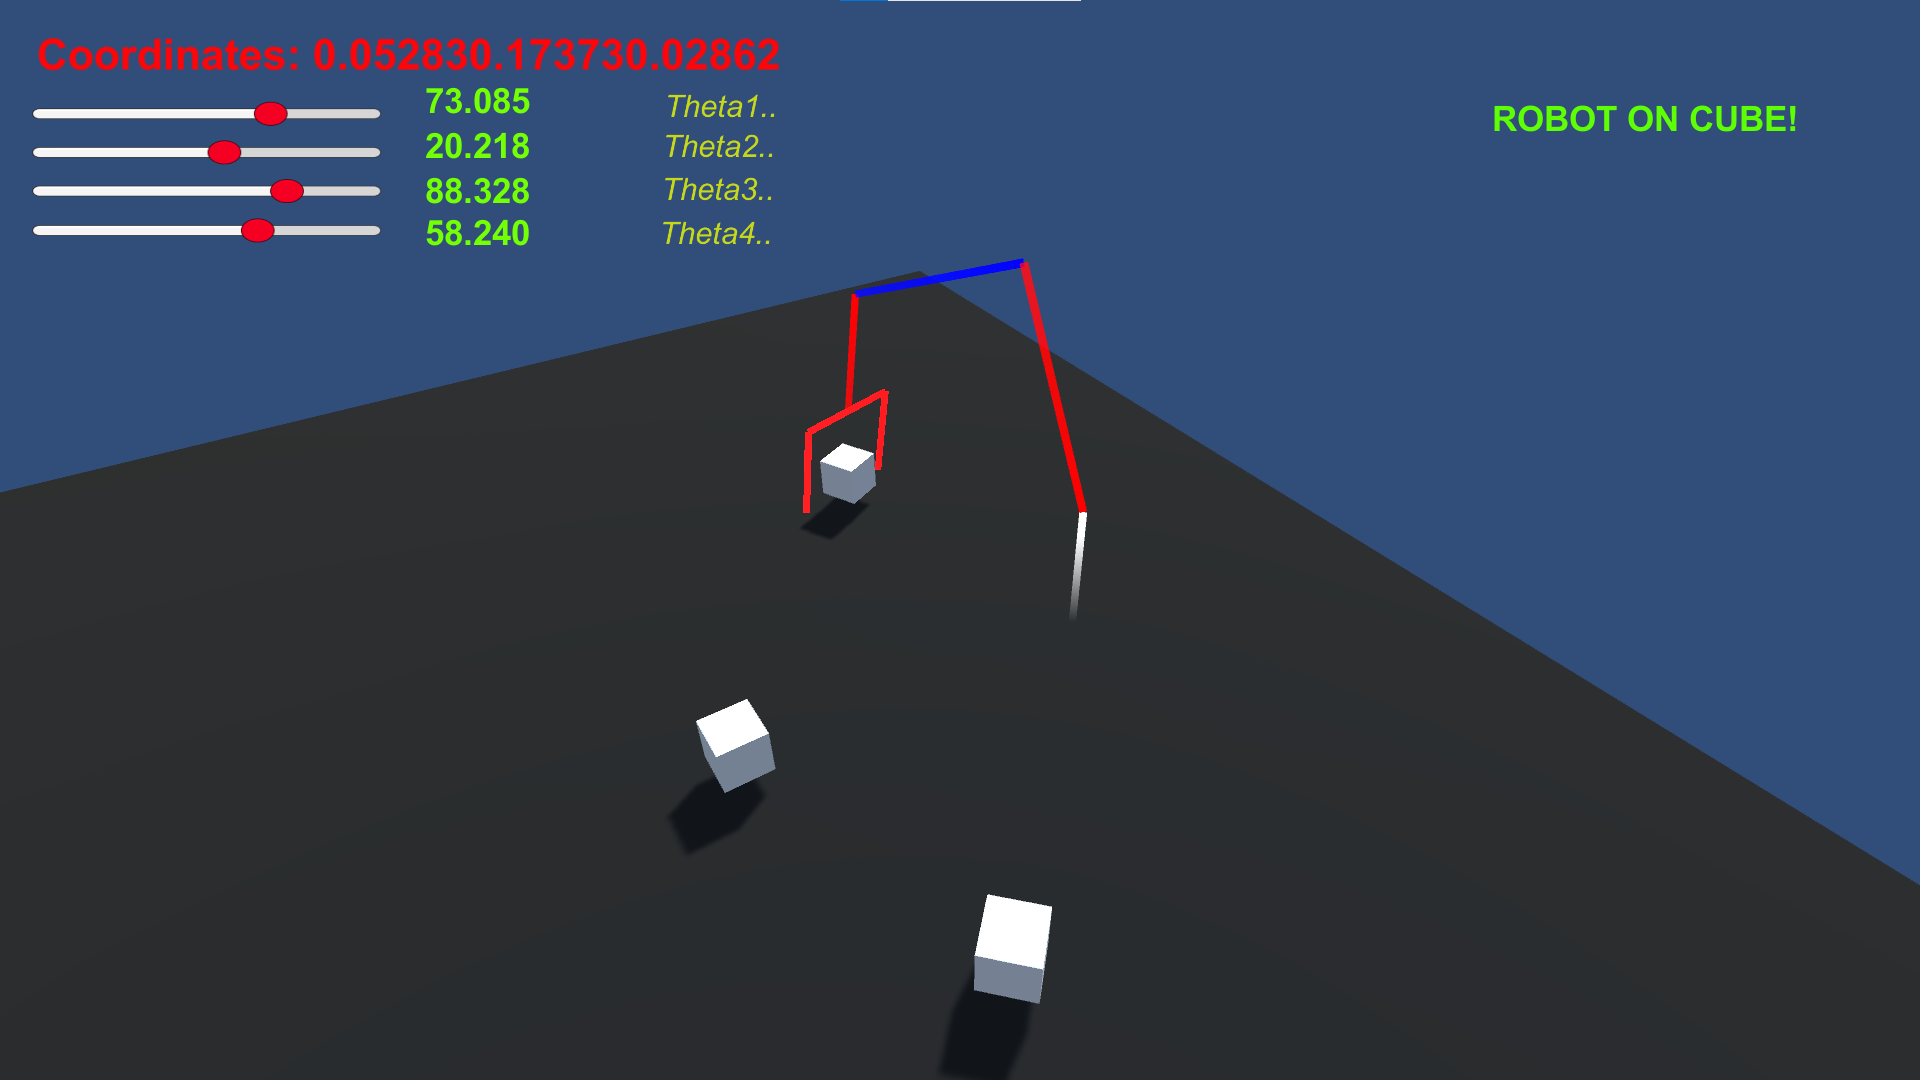
\includegraphics[width=6.5cm]{on cube.png}
    \caption{Allows user to know if the position of end effector (green dot in Figure 9) is on the cube or not}
  \end{subfigure}%
  \begin{subfigure}{.48\textwidth}
    \centering
    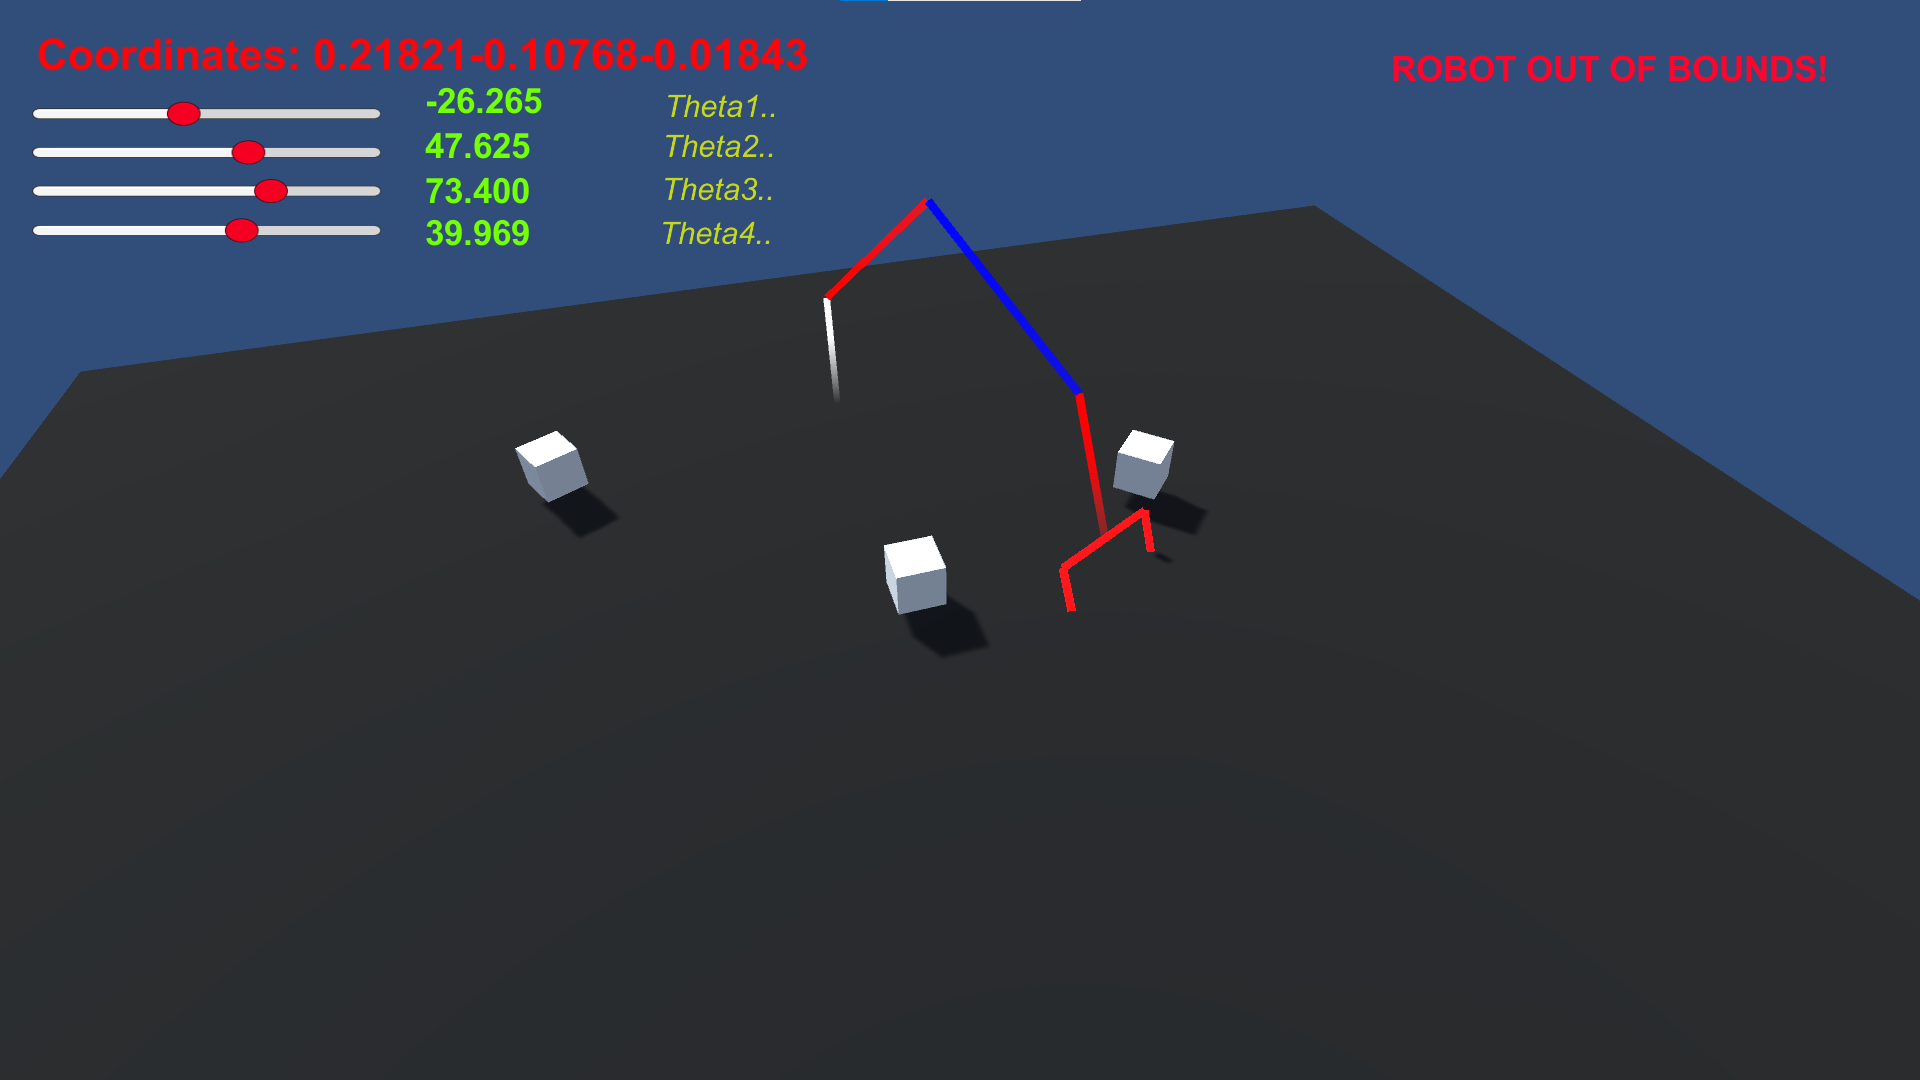
\includegraphics[width=6.5cm]{out of bounds.png}
    \caption{Checks if arm would violate the range constraints i.e. board dimensions}
  \end{subfigure}
\end{figure}

\pagebreak

\subsection{Task 2 and 3 modified DH Table}
The DH tables are modified for Task 3 and Task 4 as shown below:
  \begin{table}[h]
    \centering
    \begin{tabular}{|c|c|c|c|c|}
    \hline
    {\textbf{}} & {\textbf{$\alpha_{i-1}$}} & { \textbf{$a_{i-1}$}} & { \textbf{$d_i$}} & { \textbf{$\theta_i$}} \\ \hline
    \textbf{Waist}           & 0\degree                              & 0                        & 0.077             & $\theta_1$                \\ \hline
    \textbf{Shoulder}        & 90\degree                             & 0                        & 0                 & $\theta_2 + 90\degree  - 10.6\degree $    \\ \hline
    \textbf{Elbow}           & 0\degree                              & 0.130                    & 0                 & $\theta_3 - 90\degree  + 10.6\degree $    \\ \hline
    \textbf{Wrist}           & 0\degree                              & 0.124                    & 0                 & $\theta_4$                \\ \hline
    \textbf{Gripper}         & 0\degree                              & 0.116                    & 0                 & 0\degree                          \\ \hline
    \end{tabular}
  \end{table}

\subsection{Task 2 and 3 CAD models}
\textbf{Pen gripper}: 
Pen gripper is composed of a pair, each with the same designs but reflected.
\begin{figure}[h]
    \centering
    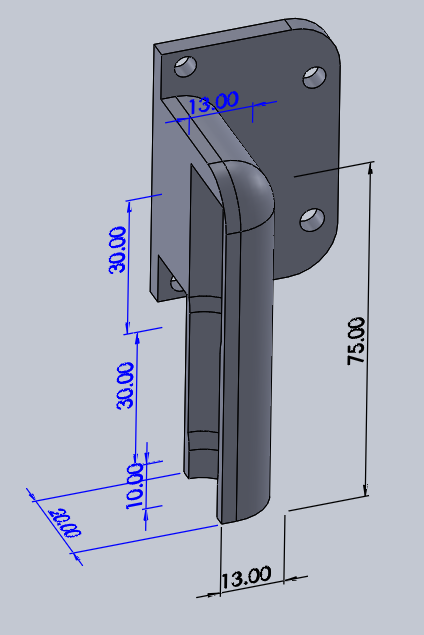
\includegraphics[width=5cm]{pen_right.png}
    \hspace{1cm}
    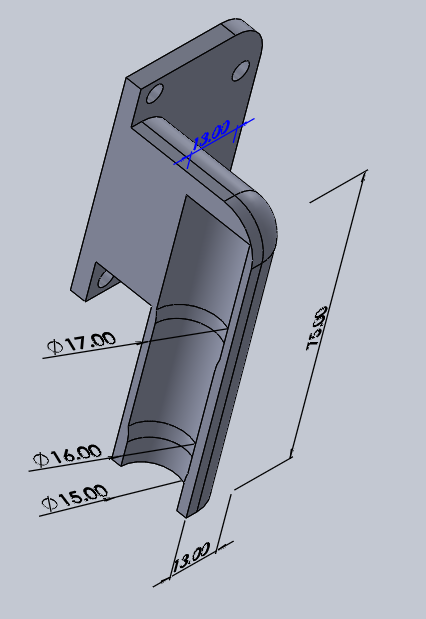
\includegraphics[width=5cm]{pen_right_2.png}
\end{figure}

\textbf{Xylophone stick gripper}: 
Xylophone stick gripper is composed of a pair, each with the same designs but
reflected.
\begin{figure}[h]
    \centering
    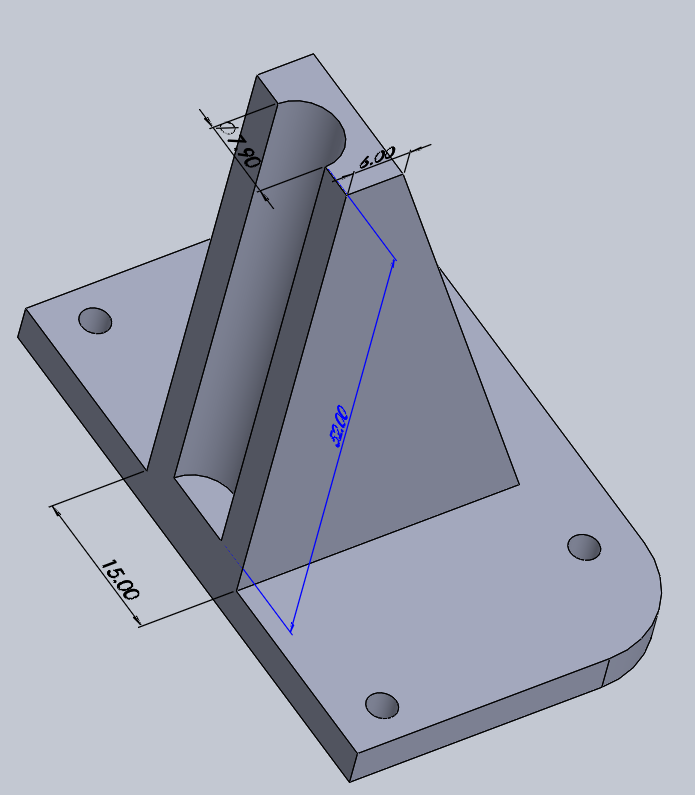
\includegraphics[width=5cm]{stick_holder.png}
\end{figure}


\pagebreak
\section{References}
\printbibliography


\end{document}